%----------------------------------------------------------------------------------------
%	PACKAGES AND OTHER DOCUMENT CONFIGURATIONS
%----------------------------------------------------------------------------------------

\documentclass[
11pt, % The default document font size, options: 10pt, 11pt, 12pt
%oneside, % Two side (alternating margins) for binding by default, uncomment to switch to one side
ngerman,
singlespacing, % Single line spacing, alternatives: onehalfspacing or doublespacing
%nolistspacing, % If the document is onehalfspacing or doublespacing, uncomment this to set spacing in lists to single
%liststotoc, % Uncomment to add the list of figures/tables/etc to the table of contents
%toctotoc, % Uncomment to add the main table of contents to the table of contents
%parskip, % Uncomment to add space between paragraphs
headsepline, % Uncomment to get a line under the header
%chapterinoneline, % Uncomment to place the chapter title next to the number on one line
%consistentlayout, % Uncomment to change the layout of the declaration, abstract and acknowledgements pages to match the default layout
]{MastersDoctoralThesis} % The class file specifying the document structure

\usepackage[latin1]{inputenc} % Required for inputting international characters. [utf8/applemac/latin1]
\usepackage[T1]{fontenc} % Output font encoding for international characters
% \usepackage[ngerman]{babel}
% \usepackage{luaotfload}
% \usepackage[EU2]{fontenc}
% \usepackage{lmodern}

\usepackage{mathpazo} % Use the Palatino font by default

\usepackage[backend=biber,style=numeric,natbib=true]{biblatex} % Use the bibtex backend with the numeric citation style, backend=bibtex

\addbibresource{quellen.bib} % The filename of the bibliography

\usepackage[autostyle=true]{csquotes} % Required to generate language-dependent quotes in the bibliography

\usepackage{siunitx} % Number formatting. [group-separator={.}]
\sisetup{group-separator = {\,}, group-minimum-digits=5}  % small spacing between every third digit of long number
% https://www.namsu.de/Extra/pakete/Siunitx.html

%----------------------------------------------------------------------------------------
%	OWN SETTINGS
%----------------------------------------------------------------------------------------

\setcounter{tocdepth}{3}  % A value of X=0 means that your table of contents will show nothing at all and 5 means, that even subparagraphs will be shown.

% Define some commands to keep the formatting separated from the content 
\newcommand{\keyword}[1]{\textbf{#1}}
\newcommand{\tabhead}[1]{\textbf{#1}}
\newcommand{\code}[1]{\texttt{#1}}
\newcommand{\file}[1]{\texttt{\bfseries#1}}
\newcommand{\option}[1]{\texttt{\itshape#1}}

%----------------------------------------------------------------------------------------
%	MARGIN SETTINGS
%----------------------------------------------------------------------------------------

\geometry{
	paper=a4paper, % Change to letterpaper for US letter
	inner=2.5cm, % Inner margin
	outer=3.8cm, % Outer margin
	bindingoffset=.5cm, % Binding offset
	top=1.5cm, % Top margin
	bottom=1.5cm, % Bottom margin
	%showframe, % Uncomment to show how the type block is set on the page
}

%----------------------------------------------------------------------------------------
%	THESIS INFORMATION
%----------------------------------------------------------------------------------------

\thesistitle{Analyse des UMAP Verfahrens} % Your thesis title, this is used in the title and abstract, print it elsewhere with \ttitle
\author{Christopher Reiners} % Your name, this is used in the title page and abstract, print it elsewhere with \author

\supervisor{Prof. Dr. Jochen Garcke}
\subject{Mathematik}
\thesistype{Bachelorarbeit}
\university{Rheinischen Friedrich-Wilhelms-Universit�t Bonn}
\department{Mathematisches Institut f�r Numerische Simulation} 
\faculty{Mathematisch-Naturwissenschaftliche Fakult�t der}
\geburtsdatum{9. April 1998}  %Author DoB
\geburtsort{Detmold}  %Author place of birth
\date{6. August 2019}  %\today  %Abgabedatum
\zweitgutachter{Dr. Bastian Bohn}



% \AtBeginDocument{
% \hypersetup{pdftitle=\thesistitle} % Set the PDF's title to your title
% \hypersetup{pdfauthor=\author} % Set the PDF's author to your name
% \hypersetup{pdfkeywords=\keywordnames} % Set the PDF's keywords to your keywords
% }

\begin{document}

\frontmatter % Use roman page numbering style (i, ii, iii, iv...) for the pre-content pages

\pagestyle{plain} % Default to the plain heading style until the thesis style is called for the body content

%----------------------------------------------------------------------------------------
%	TITLE PAGE
%----------------------------------------------------------------------------------------

\maketitle

%----------------------------------------------------------------------------------------
%	QUOTATION PAGE
%----------------------------------------------------------------------------------------

% \vspace*{0.2\textheight}

% \noindent\enquote{\itshape Do not worry about your difficulties in Mathematics. I can assure you mine are still greater.}\bigbreak

% \hfill Albert Einstein

%----------------------------------------------------------------------------------------
%	ACKNOWLEDGEMENTS
%----------------------------------------------------------------------------------------

\begin{acknowledgements}

\addchaptertocentry{\acknowledgementname} % Add the acknowledgements to the table of contents

Ich bin den Personen sehr dankbar und verbunden welche mich auch dem Weg zu dieser Arbeit begleitet haben.

Zuerst m�chte ich Annalena Lange, Lennard Schiefelbein und Nico Gerber f�r die vielen anregenden 
Gespr�che danken und Hendrik Baers und Tobias Bork, welche die letzten drei Jahre zu einer spannenden 
und herrausfordernden Studienzeit gemacht haben.

Besonderer Dank gilt Prof. Dr. Jochen Garcke f�r das sehr interessante Thema und die 
wegweisende Betreueung. Gerne m�chte ich auch Leland McInnes f�r das pers�nliche Gespr�ch in Ottawa, Kanada 
danken. So konnte ich die Motivation, welche er f�r das UMAP Verfahren hatte, aus erster Hand erfahren.

Zum Schluss meiner Familie und Freunden f�r Ihre bedingungslose Unterst�tzung.

\end{acknowledgements}

%----------------------------------------------------------------------------------------
%	LIST OF CONTENTS/FIGURES/TABLES PAGES
%----------------------------------------------------------------------------------------

\tableofcontents % Prints the main table of contents

%\listoffigures % Prints the list of figures

%\listoftables % Prints the list of tables

%----------------------------------------------------------------------------------------
%	THESIS CONTENT - CHAPTERS
%----------------------------------------------------------------------------------------

\mainmatter % Begin numeric (1,2,3...) page numbering

\pagestyle{thesis} % Return the page headers back to the "thesis" style

%!TEX root = ../main.tex

\chapter{Einleitung} 

\label{Einleitung}

% Relevanz, �bersicht, UMAP, Struktur

%----------------------------------------------------------------------------------------

%Define math commands used in this chapter
\newcommand{\R}{\mathbb{R}}  % Symbol for real numbers
\newcommand{\seqx}{\{x_i\}_{i=1}^N, \ (x_i \in \mathbb{R}^D)}  % Sequence of x_i
\providecommand{\abs}[1]{\lvert#1\rvert}  % produces | x |
\providecommand{\norm}[1]{\lVert#1\rVert}  % produces || x ||

%----------------------------------------------------------------------------------------

% N O T I Z E N
% 

% T E X T B A U S T E I N E
% 'UMAP wird f�r single cell RNA-sequencing genutzt'
% scRNA hat mehr rauschen als bulkRNA-seq und wird zur Untersuchung der genetischen 
% Information (Genexpression) einzelner Zellen genutzt.
% 'Dimension ist Anzahl der Freiheitsgerade'
% Es gibt F�lle in denen es unm�glich ist die gesamte globale Struktur zu erhalten. 
% Betrachet man beispielsweise gleichverteilte Punkte auf einem Kreis und m�chte diese 
% in R einbetten, muss es zwei Punkte geben welche getrennt werden.

%----------------------------------------------------------------------------------------
%----------------------------------------------------------------------------------------

% TODO: Was macht das Thema Dimensionsreduktion relevant?

%----------------------------------------------------------------------------------------

\section{Datenanalyse}
% Einordnung verschiedener DR Algorithmen. (Geometrie, Stochastik, Topologie)
% Was ist eine gute Repr�sentation der Daten?
% Sollte unabh�ngig von Transformationen weniger wichtiger Eigenschaften sein und 
% unterscheidbar bzgl. relevanter Eigenschaften. (evtl. Bengio zitieren)
% Fr�her 'feature engineering' jetzt lernen der wichtigen Eigenschaften (siehe Bengio 2013)
% Welche Formen von Datenanalyse (statistische, geometrische,...)

%-----------------------------------

% \subsection{Topologische Datenanalyse}
Eine neuere Form der Datenanalyse - die topologische Datenanalyse (\textit{kurz: TDA}) - 
nutzt mathematische Instrumente des Teilgebiets der Topologie 
(\textit{griechisch: Lehre vom Ort/Platz}) um Daten zu beschreiben und zu strukturieren.

Wir beschreiben die Stituation einen Datensatz $X$ zu analysieren wie folgt. Wir betrachten 
einen $D$-dimensionalen Raum und ein Objekt $K$. In unserem Fall werden wir uns gr��tenteils 
mit dem euklidischen Raum $\R^D$ versehen mit der euklidischen Norm $\norm{\cdot}$ besch�ftigen.

$K$ kann beispielsweise eine geschlossene Menge sein. Die genaue Struktur von $K$ bleibt uns allerdings unbekannt. 
Sp�ter werden wir argumentieren, dass $K$ gewisse Regularit�tseigenschaften erf�llt und 
in vielen F�llen lokal einem niedrigdimensionalen Raum $\R^d, (d \ll D)$ gleicht. 

Statt $K$ ist uns eine endliche Menge an $N$ Punkten $X=\seqx$, gegeben. 
$X$ wird als \textit{Punktwolke} bezeichnet und beschreibt in einem Experiment gemessene Daten, 
beispielsweise Sensormessdaten, biologische Informationen oder Bilddatens�tze. 

In Kapitel \ref{Experimente} werden wir uns mit einem 
Bilddatensatz mit \num{100000} Farbbildern mit einer Aufl�sung von $300 \times 300$ Pixeln 
besch�ftigen. Wir k�nnen diesen Datensatz als $N = \num{100000}$ elementige Punktwolke im 
$\R^{300 \times 300 \times 4}$ auffassen, wobei wir die vier Farbkan�le der Bilder ber�cksichtigen.

Wir gehen dabei davon aus, dass $K$ und $X$ in einem gewissen Sinne \enquote{�hnlich} sind. 
Nun ist es Ziel der TDA mittels Methoden der Topologie Aussagen �ber die Struktur von $X$ zu treffen, 
welche, aufgrund der �hnlichkeit, auch f�r $K$ gelten sollen. Die $K$ zugrundeliegende Struktur 
kann uns dann dabei helfen Aussagen �ber weitere gemessene Daten zu treffen, 
da diese auch in der uns unbekannten Menge $K$ liegen sollten. Zus�tzlich hilft
% TODO: erg�nzend siehe Oudot, Ch.4

%-----------------------------------
%----------------------------------------------------------------------------------------

% (Eher sp�ter in Kap2) Simpliziale Mengen sind einer Form um topologische R�ume kombinatoricsh darzustellen 
% deshalb eignen sie sich besonders f�r Berechnungen.

%----------------------------------------------------------------------------------------

\section{Dimensionsreduktion}

% hoch dimensionale Daten: Bilder, Word-count Vektoren, Zell Daten

% Ganz urspr�nglich Chernoff feces, dimensionen und knoten sie tSNE p.1

Sei $X=\seqx$ wir bezeichnen $D$ als die Dimension unserer Daten, beziehungsweise als die Anzahl 
der gemessenen Eigenschaften. $N$ ist die Anzahl der verf�gbaren Datenpunkte. In der Praxis k�nnen $D$ und $N$ 
sehr gro� sein. So gilt f�r den Bilddatensatz welchen wir in Kapitel \ref{Experimente} betrachten werden, 
$N=\num{100000}, D=\num{360000}$. %TODO: betrachten wir cartoonset100k oder cartoonset10k?

% Wahrscheinlichkeitstheorie:      |  Geometrie:
% Probabilistic PCA, VAEs, GANs    |  tSNE  (lt. Posada)

% Dann �berleiten zu UMAP

\textit{Hier sollen die zwei Arten an DR Algorithmen vorgestellt werden (Matrix Faktorisierung 
und Graph Layout). Zus�tzlich sollen PCA, Isomap, Laplacian Eigenmaps und t-SNE vorgestellt werden.} \\

Die meisten dimensionsreduktions Verfahren beruhen auf der Annahme, das reale hochdimensionale Daten 
sich in der Umgebung einer niedrigdimensionalen Mannigfaltigkeit konzentrieren. 
In der Literatur ist diese Annahme als Mannigfaltigkeits Hypothese (\textit{engl.: manifold hypothesis})
bekannt \cite{Mitter,Rifai}. 
Ans�tze um einen gegebenen Datensatz auf diese Annahme zu testen 
finden sich in \cite{Fefferman}.  % TODO: zu konkret?

% TODO: betone Gleichverteilung auf Mannigfaltigkeit bei UMAP

% TODO: warum ist Topologie sinnvoll?

% TODO: Betrachte Oudot s.67

% TODO: Anwendungen von persistence Oudot s.8

%----------------------------------------------------------------------------------------

\section{Eigene Beitr�ge}

Wir m�chten nun die Ziele dieser Arbeit formulieren.
\begin{itemize}
	\item Einf�hrung in die grundlegenden Werkzeuge der topologischen Datenanalyse
	\item M�gliche Schritte wie die L�cke zwischen Theorie und Praxis des UMAP Verfahrens 
		  geschlossen werden kann
	\item UMAP anhand sinnvoller Datens�tze mit anderen Dimensionsreduktionsverfahren vergleichen
	\item 
\end{itemize}
Insbesondere werden wir die in Kapitel 2 von \cite{UMAP} beschriebene Theorie ausf�hrlicher 
beschreiben und in einen allgemeineren Kontext setzen.

%----------------------------------------------------------------------------------------

\section{Gliederung}

In Kapitel \ref{Grundlagen} werden wir die theoretische Grundlage des UMAP Verfahrens erkl�ren. 
Dies wird einige Definitionen und Grundlagen aus der Kategorientheorie und der 
(Algebraischen-)Topologie erfordern. Wir haben mich bem�ht diese m�glichst vollst�ndig darzustellen.
F�r zus�tliche Informationen empfielt sich \cite{Brandenburg,Barr,Munkres}.

Kapitel \ref{UMAP} wird die Theorie des UMAP Verfahrens darstellen. Dabei werden wir 
auf die in \ref{Grundlagen} gelegten Grundlagen zur�ckgreifen. Zus�tzlich soll argumentiert 
werden, dass eine praktische Implementierung wie sie in der Theorie beschrieben ist zu 
rechenaufwendig ist und somit wenig praktischen nutzen hat. Deshalb 

%----------------------------------------------------------------------------------------

%!TEX root = ../main.tex

\chapter{Grundlagen} 

\label{Grundlagen}

%----------------------------------------------------------------------------------------

%Define math commands used just in this chapter
\renewcommand{\C}{\mathscr{C}}  % Symbol for a category C
\newcommand{\D}{\mathscr{D}}  % Symbol for a category D
\renewcommand{\N}{\mathbb{N}}  % Symbol for natural numbers
\newcommand{\M}{\mathcal{M}}  % Symbol for Manifold M
\newcommand{\cech}{\u{C}ech}  % Symbol for Cech complex
\newcommand{\Set}{\mathbf{Set}}  % Symbol for category of sets
\newcommand{\sSet}{\mathbf{sSet}}  % Symbol for category of sets
\newcommand{\Top}{\mathbf{Top}}  % Symbol for category of sets
\newcommand{\sFuzz}{\mathbf{sFuzz}}  % Symbol for fuzzy set category
\newcommand{\EPMet}{\mathbf{EPMet}}  % Symbol for category of extended pseudo metric spaces
\renewcommand{\hom}{\mathsf{Hom}}  % Symbol for morphisms
\newcommand{\fReal}{\mathsf{FinReal}}  % Symbol for Real functor
\newcommand{\fSing}{\mathsf{FinSing}}  % Symbol for Sing functor
\newcommand{\fsFuzz}{\mathbf{Fin\text{-}sFuzz}}  % Symbol for finite fuzzy set category
\newcommand{\fEPMet}{\mathbf{Fin\text{-}EPMet}}  % Symbol for category of finite extended pseudo metric spaces
\newcommand*{\Scale}[2][4]{\scalebox{#1}{\ensuremath{#2}}}
\newcommand{\tConorm}{\Scale[1.5]{\bot}^N_{i=1}}  % Symbol for t-Conorm, $\bot_{\{1 \leq i \leq N\}}$ $\underset{i=1}{\overset{N}{\bot}}$ $\bot^N_{i=1}$

%----------------------------------------------------------------------------------------

% Struktur Posada:
% Kategorientheorie (Kategorien, Funktoren, nat�rliche Transformationen)
% Dieses allgemeine Ger�st l�sst einen leicht simpliziale Komplexe zu simplizialen Mengen
% veralgemeinern, unischere Mengen einf�hren und die f�r UMAP verwendete Theorie erl�utern.
% discrete, free and monoid category
% category Set, Top, duale Kategorie kurz (morphismen umkehren)

% Zusammenfassen der bisherigen Konstruktion und das man einen Schritt weiter geht
% Ausblicke auf das was man sp�ter mit einer Definition macht
% Wof�r war die gerade gemachte Definition sinnvoll
% Die Definition einer Adjunktion ist daf�r wichtig einen zwischen metrischen R�umen und 
% unscharfen simplizialen Mengen zu �bersetzen.
% Typische Verwendungen f�r die Definition

% TODO: Daniel 
% Section 2:
% Section 2.2: Man k�nnte noch zitieren in welchem Paper Samuel Eilenberg und Saunders Mac Lane Kategorientheorie eingef�hrt haben.

% Bemerkung �ber Klassen: Ich w�rde den Satz "Eine Klasse ist eine Menge, die zu gro� ist um eine Menge zu sein." �ndern. Evtl. sowas wie: Bei Klassen kann es sich um Ansammlungen von Objekten handeln, die "gr��er" als Mengen sind.

% Bei der Definition des Kompositionsoperators f�r die duale Kategorie steht ein Hom(C,B) zu viel da.

% Bei der Definition vom n-Simplex: Facetten sind glaub ich die Mengen die von Teilmengen von {v_0,...,v_n} aufgespannt werden und nicht die Teilmengen selbst oder?

% Bei der Definition von abstrakten Simplizialkomplexen: Das mit den (i+1)-elementigen Teilmengen sieht irgendwie falsch aus, bzw. man versteht nicht wirklich was du meinst. 
% 														Das w�rde doch hei�en, dass jeder Punkt aus z.b. S^1 auch in S^0 ist (?)

%----------------------------------------------------------------------------------------
%----------------------------------------------------------------------------------------

% \section{Einleitung}
	Das UMAP Verfahren entstammt dem Gebiet der topologischen Datenanalyse. Die Theorie f�r das Verfahren 
	nutzt Grundlagen aus den Bereichen der (algebraischen) Topologie, Kategorientheorie und Mengentheorie. 
	Wir wollen diese nun einf�hren. Dazu geben wir die wichtigsten Definitionen und S�tze und werden 
	diese anschaulich erkl�ren und in den Rahmen des UMAP Verfahren fassen. % TODO: ?erw�hne appendixA

	Die grundlegenden Definitionen \textit{topologischer und metrischer R�ume} in Abschnitt \ref{seq:top} 
	werden uns helfen \textit{(riemannsche) Mannigfaltigkeiten} einzuf�hren. Der Begriff der Mannigfaltigkeit 
	formalisiert den niedrigdimensionalen Raum auf welchem der zu untersuchende Datensatz $X$ liegt.

	Die geometrische und topologische Struktur dieser R�ume sollen durch \textit{simpliziale Mengen} dargestellt 
	werden. Um diese in Abschnitt \ref{seq:sSet} einzuf�hren, ben�tigen wir grundlegende Definitionen 
	aus der Kategorientheorie, siehe dazu Abschnitt \ref{seq:cat}.

	In Abschnitt \ref{seq:fuzz} werden \textit{unscharfe Mengen} eingef�hrt, diese werden in Kapitel \ref{UMAP} ben�tigt 
	um der topologischen Repr�sentation der Daten $X$ eine metrische Struktur zu verleihen.

%----------------------------------------------------------------------------------------

\section{Topologische R�ume} \label{seq:top}
	Der Grundlegende Begriff der Topologie ist der des topologischen Raumes.

	\begin{defn} %[Topologischer Raum]
		Sei $X$ eine nichtleere Menge. Ein Mengensystem $\tau \subset \mathcal{P}(X)$ hei�t \textit{Topologie auf X}, 
		falls die folgenden drei Bedingungen erf�llt sind: 

		\begin{enumerate}
			\item $\emptyset, X \in \tau$,
			\item die Vereinigung beliebig vieler Mengen aus $\tau$ liegt wieder in $\tau$,
			\item sind $U, V \in \tau$, so liegt auch der Durchschnitt $U \cap V$ in $\tau$.
		\end{enumerate}

		Das Paar $(X,\tau)$ hei�t \textit{topologischer Raum}. Die Mengen $U \in \tau$ nennt man \textit{offene} Mengen 
		des topologischen Raumes.
	\end{defn}

	\begin{rem}
		Wenn die Topologie $\tau$ eines topologischen Raumes $(X,\tau)$ aus dem Kontext klar ist, wird diese nicht explizit erw�hnt.
	\end{rem}

	Man kann den Begriff erweitern indem man einen Abstandsbegriff auf der Menge $X$ definiert. Dies f�hrt uns 
	zum metrischen Raum.

	\begin{defn} %[Metrischer Raum]
		Sei $X$ eine nichtleere Menge. Eine Abbildung $d:X \times X \to \R_{\geq 0}$ hei�t \textit{Metrik} auf $X$, falls f�r beliebige Elemente 
		$x, y, z \in X$ die folgenden drei Bedingungen erf�llt sind:

		\begin{enumerate}
			\item $d(x,y) = 0 \iff x = y$,
			\item $d(x,y) = d(y,x)$,
			\item $d(x,y) \leq d(x,z) + d(z,y)$.
		\end{enumerate}

		Das Paar $(X, d)$ hei�t \textit{metrischer Raum}. Die Metrik $d$ hei�t \textit{Pseudometrik}, wenn die erste Bedingung durch 
		$d(x,y) = 0 \Leftarrow x = y$ abgeschw�cht wird.

		Falls die Metrik den Wert $\infty$ annehmen kann, sprechen wir von einer \textit{erweiterten Metrik}.
	\end{defn}

	\begin{rem}
		In Fakt ist die Erweiterung einer Metrik um den Wert $\infty$ keine Einschr�nkung. F�r eine gegebene erweiterte Metrik $d$ 
		kann n�mlich stets �quivalente eine (echte) Metrik $d'$ konstruiert werden, zum Beispiel ist $d' = \frac{d}{1+d}$ �quivalent 
		zu einer erweiterten Metrik $d$. Eine formale Definition der �quivalenz zweier metrischer R�ume soll hier nicht gegeben werden. 
		Es gen�gt zu wissen, dass wichtige topologische Eigenschaften erhalten zwischen den beiden R�umen �bertragen werden k�nnen.
		Hier gilt $x + \infty = \infty + x = \infty, x \in [0,\infty]$.
	\end{rem}

	% https://math.stackexchange.com/questions/399722/metric-assuming-the-value-infinity#399759 erweiterte metriken beitzten gute eigenschaften

	% TODO: n-dim euklidischer Raum als Beispiel

	% nichtexpansive Abbildung

	\begin{rem}
		F�r einen metrischen Raum $(X, d)$, ist ein offener \textit{Ball mit Radius $r > 0)$} und Mittelpunkt $p$ mit $p$ aus $X$ gegeben durch: 
		
		\begin{align}
			B_r(p) \coloneq \{x \in X | d(x,p) < r\}.
		\end{align}

		F�r den Fall, das $X$ der $n$-dimensionale euklidische Raum ist, ist das $n$-dimensionale Volumen bez�glich der euklidischen Metrik:

		\begin{align}
			V_n(B_r(p)) = \frac{\pi^{\frac{n}{2}}}{\Gamma(\frac{n}{2}+1)}r^n
		\end{align}
	\end{rem}

	In der Einleitung bereits erw�hnt, werden wir Annehmen, dass unsere Daten $X=\{\mathbf{x}_i\}_{i=1}^N, (\mathbf{x}_i \in \R^D)$ mit $D$ 
	gemessenen Eigenschaften mittels $d, (d \ll D)$ Eigenschaften dargestellt werden k�nnen. 
	Um dies in die Sprache der Topologie zu fassen, werden wir den Begriff der \textit{Mannigfaltigkeit} ben�tigen.
	Anschaulich ist eine $d$-dimensionale Mannigfaltigkeit ein topologischer Raum welcher lokal dem euklidischen Raum $\R^d$ gleicht.
	Bevor wir Mannigfaltigkeiten einf�hren ben�tigen wir \textit{hom�omorphe Abbildungen}.

	\begin{defn} %[Hom�omorphimus]
		Seien $X$ und $Y$ topologische R�ume. Eine Abbildung $f:X \to Y$ ist ein \textit{Hom�omorphismus}, wenn gilt:
		
		\begin{enumerate}
			\item $f$ ist bijektiv,
			\item $f$ ist stetig also, wenn die Urbilder offener Mengen wieder offen sind,
			\item die Umkehrfunktion $f^{-1}$ ist ebenfalls stetig.
		\end{enumerate}

		Wenn ein Hom�omorphismus $f:X \to Y$ gibt, so nennen wir $X$ und $Y$ \textit{hom�omorph}.
	\end{defn}
	
	\begin{defn} %[Mannigfaltigkeit]
		Sei $\M$ ein topologischer Raum, $d \in \N$, er hei�t \textit{$d$-dimensionale Mannigfaltigkeit}, 
		wenn folgende drei Bedingungen erf�llt sind:

		\begin{enumerate}
			\item f�r alle paarweise verschiedenen Punkte $p, q \in \M$ existieren disjunkte offene Mengen $U, V \subseteq \M$ 
				  mit $p \in U$ und $q \in V$,
			\item die Topologie von $\M$ besitzt eine abz�hlbare Basis 
			\item jeder Punkt in $\M$ besitzt eine Umgebung, die hom�omorph zu einer offenen Teilmenge des $\R^d$ ist.
		\end{enumerate}
	\end{defn}

	Um eine \textit{riemannsche Mannigfaltigkeit} definieren zu k�nnen, ben�tigen wir noch einige Definitionen. 

	\begin{defn} %[Diffeomorphismus]
		Eine Abbildung $f:U\to V$ zwischen offenen Mengen $U, V \subset \R^n$ hei�t \textit{$C^k$-Diffeomorphismus}, falls
		\begin{enumerate}
			\item $f$ ist bijektiv 
			\item $f$ ist �berall $k$-mal stetig differenzierbar
			\item die Umkehrabbildung $f^{-1}$ ist �berall $k$-mal stetig differenzierbar.
		\end{enumerate}
	\end{defn}

	\begin{defn} %[Karte]
		Es sein $\M$ eine Mannigfaltigkeit der Dimension $d$. Eine \textit{Karte} auf $\M$ ist ein Paar $(U, \phi)$, wobei $U \subseteq \M$ 
		eine offene Menge und $\phi : U \to \phi(U)$ ein Hom�omorphismus mit $\phi(U) \subseteq \R^d$ ist.

		Sind $(U, \phi)$ und $(V, \psi)$ zwei Karten von $\M$ mit $U \cap V \neq \emptyset$, so nennt man die Abbildung 
		\begin{align}
			\psi \circ \phi^{-1} : \phi(U \cap V) \to \psi(U \cap V)
		\end{align}
		einen \textit{Kartenwechsel}. 

		Ein \textit{Atlas} f�r $\M$ ist dann eine Familie $(U_i,\phi_i)_{i \in I}$ von Karten, so dass $\M = \cup_{i \in I} U_i$ gilt. 
		Man nennt einen Atlas \textit{$C^k$-differenzierbar} mit $k \geq 1$, wenn alle seine Kartenwechsel $C^k$-Diffeomorphismen sind.
	\end{defn}

	Karten werden genutzt um zwischen der Mannigfaltigkeit und dem $\R^d$ zu �bersetzen. 

	\begin{figure}
		%\centering
		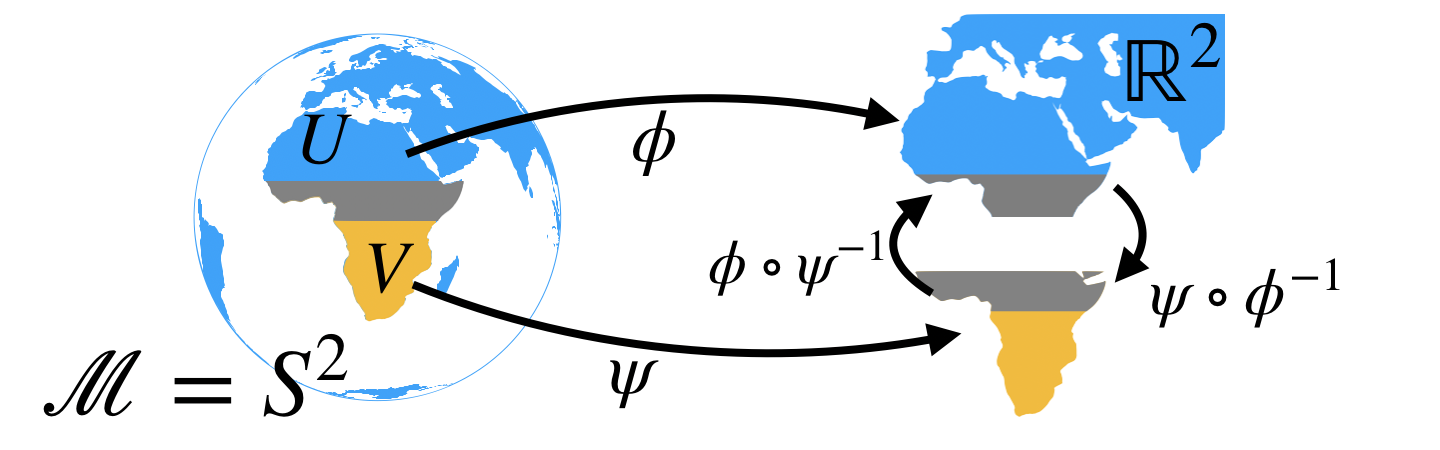
\includegraphics[width=400px, height=125px]{Figures/Atlas}
		%\decoRule
		\caption[Atlas einer Mannigfaltigkeit]{Atlas einer Mannigfaltigkeit.}
		\label{fig:Atlas}
	\end{figure}

	\begin{defn}

		Eine \textit{differenzierbare} Mannigfaltigkeit ist eine...
	\end{defn}

	\begin{ex}
		$S^n$ ist eine $n$-dimensionale Mannigfaltigkeit im $\R^{n+1}$.
	\end{ex}

	% TODO: weiteres Beispiel

	Nun k�nnen wir im Fall der Dimensionsreduktion die Vermutung aufstellen, dass unsere Daten $X$ auf einer 
	$d$--dimensionale Mannigfaltigkeit $\M$ im $\R^D$ liegen. Zus�tzlich gehen wir davon aus, dass unsere Daten 
	einen Abstandsbegriff erlauben. Somit l�sst sich die Definition der Mannigfaltigkeit erweitern.

	% TODO: Definition riemannsche Mannigfaltigkeit, erw�hne matrix darstellungs
	\begin{defn}[Riemannsche Mannigfaltigkeit]
		Sei $g$,...

		Ein Tupel $(\M, g)$, wobei $\M$ eine Mannigfaltigkeit und $g$ eine riemannsche Metrik ist hei�t
		\textit{riemannsche Mannigfaltigkeit}.
	\end{defn} 

	% TODO: Metrisierbarkeit riemannsche Mannigfaltigkeit
	\begin{rem}
		Eine riemannsche Mannigfaltigkeit ist stets metrisierbar im Sinne, das ...
	\end{rem}

	% TODO: Beispiele riemannsche Mannigfaltigkeit

	Die Riemannmetrik beschreibt eine Distanz auf der Mannigfaltigkeit. Die L�nge eines k�rzesten Weges auf $\M$ 
	zwischen zwei Punkten $p, q \in \M$ wird als Geod�te bezeichnet und ist definiert als 

	\begin{defn}[Geod�te]
		Seien $p, q \in \M$ ...
	\end{defn}

	Der Begriff der riemannschen Mannigfaltigkeit erm�glicht es uns unsere zentrale Annahme, das $X \subseteq \R^D$ 
	einer niedrigdimensionalen Struktur entnommen ist, zu formalisieren.
	Wir m�chten nun diese niedrigdimensionale Struktur genauer beschreiben.

%----------------------------------------------------------------------------------------

\section{Kategorientheorie} \label{seq:cat}
	Die f�r die mathematischen Grundlagen des UMAP Verfahren ben�tigten Definitionen 
	werde ich mithilfe der Kategorientheorie einf�hren. 
	Diese sehr abstrakte Form mathematische Objekte und Zusammenh�nge zu formalisieren 
	wurde erstmals in den vierziger Jahren von Samuel Eilenberg und Saunders Mac Lane eingef�hrt. \\
	Die Definitionen sind dem Buch von Brandenberg \cite{Brandenburg} entnommen. 
	 
	\begin{defn}[Kategorie]
	 Eine Kategorie $\C$ besteht aus folgenden Daten:
	 	\begin{enumerate}
	 		\item Eine Klasse $Ob(\C)$, deren Elemente wir \textit{Objekte} nennen
			\item zu je zwei Objekten $\mathit{A, B \in Ob(\C)}$ einer Menge $\mathit{\hom_\C(A, B)}$, 
				deren Elemente wir mit $f: A \to B$ notieren und \textit{Morphismen} von $A$ nach $B$
				nennen,
			\item zu je drei Objekten $A, B, C \in Ob(\C)$ einer Abbildung
				\begin{equation*}
					\hom_\C(A, B) \times \hom_\C(B, C) \to \hom_\C(A, C)
				\end{equation*}
				die wir mit $(f, g) \mapsto g \circ f$ notieren und \textit{Komposition von Morphismen} nennen,
			\item zu jedem Objekt $A \in Ob(\C)$ einen ausgezeichneten Morphismus
				\begin{equation*}
					id_A \in \hom_\mathcal{C}(A,A),
				\end{equation*}
				welchen wir die \textit{Identit�t} von $A$ nennen.
		\end{enumerate}
	 Diese Daten m�ssen den folgenden Regeln gen�gen:
		\begin{enumerate}
			\item Die Komposition von Morphismen ist \textit{assoziativ}: F�r drei Morphismen 
				der Form $f:A \to B, \ g:  B \to C, \ h:C \to D$ in $\C$ gilt
				\begin{equation*}
					h \circ (g \circ f) = (h \circ g) \circ f
				\end{equation*}
				als Morphismen $A \to D$.
			\item Die Identit�t sind \textit{beidseitig neutral} bez�glich der Komposition:
				F�r jeden Morphismus $f: A \to B$ in $\C$ gilt
				\begin{equation*}
					f \circ id_A =  f = id_A \circ f
				\end{equation*}
		\end{enumerate}
	\end{defn}

	\begin{rem}
		Anstelle von $A \in Ob(\C)$ schreibt man meistens $A \in \C$. 
		Falls die Kategorie $\C$ aus dem Kontext bekannt ist, werden wir $\hom_\C(A, B)$
		mit $\hom(A, B)$ abk�rzen.
	\end{rem}

	\begin{rem}
		% TODO: Besser formulieren
		Eine Klasse ist eine Menge, welche zu gro� ist um eine Menge zu sein. 
		F�r eine Definition einer Klasse verweisen wir auf \cite{Levy}. 
		In unseren Beispielen gen�gt die Vorstellung einer Menge.
		Meist ist $Ob(\C)$ sogar eine Menge. Dann spricht man formal von einer strikten kleinen Kategorie.
	\end{rem}

	\begin{ex}
		\textit{Passende Beispiele von Kategorien, welche sp�ter wieder genutzt werden. $\Top, \Set, (Fin)EPMet$} 
		% Erw�hne dass nicht erweiternde Abbildungen genutzt werden, da Isometrien der R�ume zu restriktiv w�ren 
	\end{ex}

	Ein weiterer f�r die folgenden Definitionen wichtiger Begriff ist der der dualen Kategorie.

	\begin{defn}[Duale Kategorie]
		Es sei $\C$ eine Kategorie. Dann k�nnen wir eine neue Kategorie $\C^{op}$	 konstruieren: 
		Sie besitzt dieselben Objekte wie $\C$, allerdings werden die Morphismen \enquote{umgedreht}:
		F�r $A,B \in \C$ sei
		\begin{equation*}
			\hom_{\C^{op}}(A, B) \coloneqq \hom_\C(B, A).
		\end{equation*}
		Die Identit�ten ver�ndern sich nicht. Die Komposition
		\begin{equation*}
			\circ^{op} : \hom_{\C^{op}}(A, B) \times \hom_{\C^{op}}(B, C) \to \hom_{\C^{op}}(A, C) 
		\end{equation*}
		ist durch
		\begin{equation*}
			\hom_\C(B, A) \times \hom_\C(C, B) \cong \hom_\C(C, B) \times \hom_\C(C, B) \times \hom_\C(B, A) \mathring{\longrightarrow} \hom_\C(C, A)
		\end{equation*}
		definiert, d.h. $f \circ^{op} g \coloneqq g \circ f$. Auf diese Weise ist  $\C^{op}$ tats�chlich 
		eine Kategorie und hei�t die \textit{zu} $\C$ \textit{duale Kategorie}.
	\end{defn}

	\begin{rem}
		Eine Eigenschaft der dualen Kategorie ist, dass Aussagen, 
		welche f�r alle Kategorien bewiesen wurden, auch f�r alle dualen Kategorien gelten. 
	\end{rem}

	Wir m�chten nun den Begriff des Funktors zwischen zwei Kategorien einf�hren. Ein Funktor ordnet Objekte einer 
	Kategorie $\C$ Objekten einer Kategorie $\D$ zu, und entsprechend f�r Morphismen. Insbesondere bleibt 
	die Eigenschaft der Isomorphie zwischen zwei Objekten erhalten. 
	%TODO: Was ist ein isomorpher Funktor?

	\begin{defn}[Funktor]
		Es seien $\C$ und $\D$ zwei Kategorien. Ein \textit{Funktor}
		\begin{equation*}
			F : \C \to \D
		\end{equation*}
		von $\C$ nach $\D$ besteht aus folgenden Daten:
		\begin{enumerate}
			\item f�r jedes Objekt $A \in \C$ ein Objekt $F(A) \in \D$,
			\item f�r jeden Morphismus $f: A \to B$ in $\C$ einen Morphismus
						\begin{equation*}
							F(f) : F(A) \to F(B)
						\end{equation*}
						in $\D$.
			\end{enumerate}
		Dabei soll gelten:
		\begin{enumerate}
			\item F�r jedes Objekt $A \in \C$ ist $F(id_A) = id_{F(A)}$.
			\item F�r je zwei Morphismen $f: A \to B,\ g: B \to C$ in $\C$ gilt in $\D$:
						\begin{equation*}
							F(g \circ_{\C} f) = F(g) \circ_{\D} F(f)
						\end{equation*}
		\end{enumerate}
	\end{defn}

	\begin{rem}
		Bez�glich der Kategorie $\C$ ist ein Funktor $F : \C \to \D$ kovariant, w�hrend 
		$F : \C^{op} \to \D$ kontravariant (bzgl. $\C$) ist.
	\end{rem}

	\begin{rem}
		Insbesondere kann man f�r eine Kategorie $\C$ und Objekte $A, B, C \in \C$ den \textit{Hom-Funktor} 
		definieren, indem man 

		\begin{equation}
			\label{Hom-Funktor}
			\hom(-,B): \C \to \Set
		\end{equation}

		betrachtet. Der Hom-Funktor bildet ein Objekt $A \in \C$ auf die Menge der Morphismen $\hom(A, B)$ ab, 
		und einen Morphismus $h: A \to C$ auf die Funktion 

		\begin{equation}
			\hom(h, B): \hom(C, B) \to \hom(A, B), \text{wobei } g \mapsto g \circ h \text{ f�r } g \in \hom(C, B)	
		\end{equation}

	\end{rem}

	Eine h�ufig verwendete Form eines kontravarianten Funktors ist die Pr�garbe 
	(\textit{engl.: presheaf}). Wir werden diesen Funktor sp�ter verwenden um 
	\textit{simpliziale Mengen} einzuf�hren. % TODO: weglassen oder genauer beschreiben?

	\begin{defn}[Pr�garbe]
		Eine Pr�garbe auf einer kleinen Kategorie $\C$ ist ein Funktor
		\begin{equation*}
			F: \C^{op} \to \Set
		\end{equation*}
		von der dualen Kategorie $\C^{op}$ von $\C$ in die Kategorie $\Set$ von Mengen.
	\end{defn}

	\begin{defn}[Pr�garbenkategorie]
		Sei $\widehat{\C}$ die Pr�garbenkategorie einer Kategorie $\C$ : Objekte sind die 
		Funktoren $F: \C^{op} \to \Set$, und Morphismen sind nat�rliche 
		Transformationen der Funktoren.
	\end{defn}

	% TODO: wird dies ben�tigt?
	\begin{rem}
		Allgemeiner kann man auch die Kategorie $[\C, \D]$ einf�hren, deren Objekte 
		Funktoren $F: \C \to \D$ sind und deren Morphismen ebenfalls nat�rliche 
		Transformationen der Funktoren sind.
	\end{rem}


	% TODO: Definiere nat�rliche Transformationen. 
	% https://ncatlab.org/nlab/show/natural+transformation

	\begin{YL}
		Random Text
		% TODO: add Yoneda lemma
	\end{YL}

	\begin{defn}[Adjunktion]
		% TODO: f�ge Definition einer Adjunktion ein
	\end{defn}

%----------------------------------------------------------------------------------------

\section{Simpliziale Mengen} \label{seq:sSet}
	F�r die Konstruktion der topologischen Repr�sentation der Daten werden wir \textit{simpliziale Mengen} 
	ben�tigen. Diese stellen eine Verallgemeinerung der in der TDA h�ufig verwendeten \textit{Simplizialkomplexe} 
	dar. Wir m�chten den interessierten Leser an dieser Stelle auf die sehr verst�ndlich und ausf�hrlich gestalteten 
	Notizen von Friedman \cite{Friedman} verweisen, dort wird der Unterschied zwischen diesen beiden Konstrukten 
	sehr illustrativ erl�utert. % TODO: Appendix mit Zusammenfassung? 

	Um simpliziale Mengen einzuf�hren werden wir die kategorientheoretische Definition verwenden. 
	Daf�r wird die \textit{Simplexkategorie} ben�tigt. Zuerst werden wir der Vollst�ndigkeit halber die Definition eines 
	\textit{geometrischen Simplex} geben.

	\begin{defn} %[(geometrischer) Simplex]
		Ein \textit{(geometrischer) $n$-Simplex} ist eine von $n+1$ geometrisch unabh�ngigen Punkten $\{v_0,\dotsc,v_n\}$ 
		aufgespannte konvexe H�lle im euklidischen Raum. Die geometrische Unabh�ngigkeit der Vektoren bedeutet dabei, das 
		$v_1 - v_0, \dotsc v_n - v_0$ linear unabh�ngig sind. 
		Die Vektoren $v_i$ werden \textit{Knoten} genannt und die Teilmengen von $\{v_0,\dotsc,v_n\}$, 
		\textit{Facetten} des $n$-Simplex.
	\end{defn}

	\begin{defn}[Simplexkategorie]
		Die Objekte der \textit{Simplexkategorie} $\Delta$ sind die Mengen 
		$[n] \coloneqq \{0,1,\dotsc,n\}$ f�r $n \in \mathbb{N}$, 
		und Morphismen sind monoton wachsende Abbildungen. 

		Dabei ist $[n] \coloneqq \{1,\dotsc,n\}$.
	\end{defn}

	\begin{figure}
		%\centering
		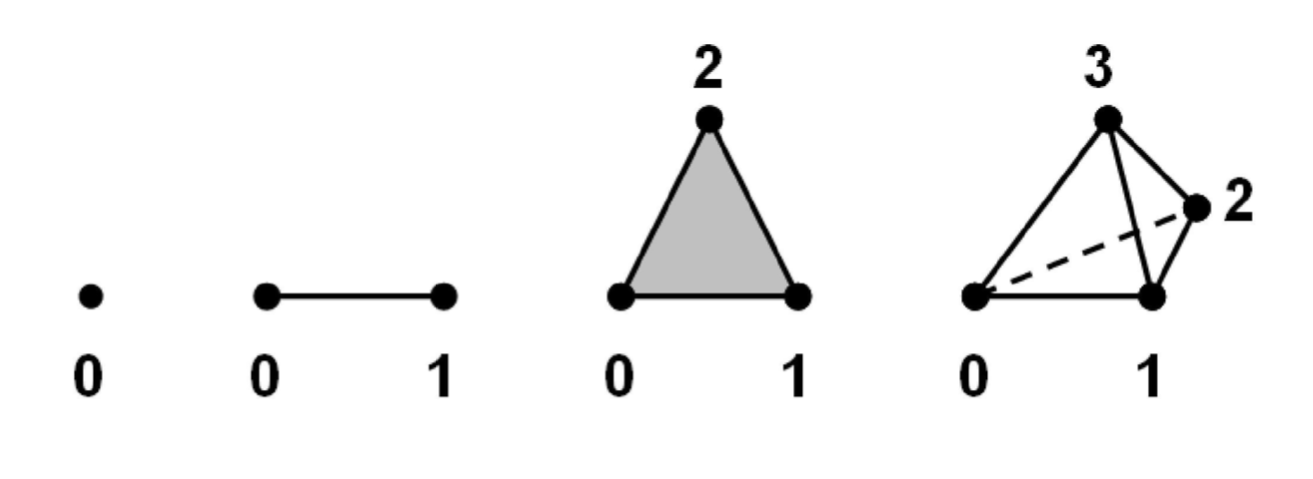
\includegraphics[width=400px, height=146px]{Figures/geom_simplizes}
		%\decoRule
		\caption[Geometrische Simplizes]{Die geometrischen 0-, 1-, 2- und 3-Simplizes, 
				in manchen F�llen werden diese auch als (geordnete) Standardsimplizes bezeichnet.}
		\label{fig:geom_simplizes}
	\end{figure}

	Um eine Verbindung zwischen der Simplexkategorie und geometrischen $n$-Simplizes (siehe Abbildung \ref{fig:geom_simplizes}) herzustellen, 
	betrachtet man die $n$-elementigen Mengen in $\Delta$ und den Funktor $\abs{\cdot}: \Delta \to \Top$, 
	gegeben durch

	\begin{equation*}
		\abs{\cdot} : [n] \mapsto \abs{\Delta^n} \coloneqq \biggl\lbrace (t_0, \dotsc, t_n) \in \R^{n+1} 
		\Big\vert \sum_{i=0}^n t_i = 1, t_i \geq 0 \biggr\rbrace
	\end{equation*}

	Das Bild von $[n]$ unter $\abs{\cdot}$ ist somit ein geometrischer $n$-Simplex.

	\begin{defn}
		Eine \textit{simpliziale Menge} ist ein Funktor 
		$X : \Delta^{op} \to \Set$. �blicherweise wird 
		$X([n])$ als $X_n$ geschrieben, und wir bezeichnen die Elemente $x \in X_n$ als n-Simplizes. 
		Der n-dimensionale \textit{Standardsimplex} ist 
		
		\begin{equation*}
			\Delta^n \coloneqq \hom(-, [n]).
		\end{equation*}
	\end{defn}

	\begin{rem}
		Simpliziale Mengen sind also Hom-Funktoren (siehe Gleichung (\ref{Hom-Funktor})).
	\end{rem}

	% TODO: Alternative Definition simplizialer Mengen

	\begin{defn}
		Die Objekte der Kategorie der simplizialen Mengen $\sSet$ sind simpliziale Mengen und ihre Morphismen sind nat�rliche Transformationen.
	\end{defn}

	Um ein besseres Verst�ndnis f�r eine simpliziale Menge zu bekommen ist es oft sinnvoll an einen \textit{Simplizialkomplex} 
	zu denken. 

	\begin{defn} %[Simplizialkomplex]
		Ein \textit{(geometrischer) Simplizialkomplex} $\mathcal{K}$ in $\R^n$ ist eine Menge von (geometrischen) Simplizes, 
		m�glicherweise unterschiedlicher Dimension, in $\R^n$, so dass
		\begin{enumerate}
			\item jede Facette eines Simplex aus $\mathcal{K}$ in $\mathcal{K}$ ist, und
			\item der Schnitt zweier Simplizes aus $\mathcal{K}$ ist eine Facette beider Simplizes.
		\end{enumerate}
	\end{defn}

	\begin{rem}
		Ein Simplizialkomplex ist anschaulich betrachtet ein geometrisches Objekt, welches aus mehreren Simplizes \textit{zusammengef�gt} wird. 
		Die Simplizes d�rfen dabei nur entlang ihrer Facetten \textit{zusammengef�gt} werden. 
	\end{rem}

	Ein Simplizialkomplex kann dabei helfen einen topologischen Raum zu beschreiben, die kombinatorische Struktur des 
	Simplizialkomplexes kann dann dazu genutzt werden Aussagen �ber den zugrundeliegenden topologischen Raum zu treffen. 
	Dabei sind die genauen r�umlichen Lagebeziehungen der Simplizes oft zu vernachl�ssigen und es kann folgende Verallgemeinerung gemacht werden:  

	\begin{defn} %[Abstrakter Simplizialkomplex]
		Ein \textit{abstrakter Simplizialkomplex} besteht aus einer Menge $S^0$ an \textit{Knoten} und, f�r jedes $k$, einer Menge $S^k$, bestehend aus 
		Teilmengen von $S^0$ der Kardinalit�t $k+1$, so dass jede $(i+1)$-elementige Teilmenge einer Menge aus $S^k$ auch in $S^i$ ist.
		Die Menge $S^k$ wird \textit{$k$-Skelett} genannt.
	\end{defn}

	\begin{rem}
		Analog zum $k$-Skelett eines Simplizialkomplexes werden wir im folgenden die $k$-Simplizes einer simplizialen Menge als $k$-Skelett bezeichnen. 
		F�r simpliziale Mengen wird diese Bezeichnung nicht konsistent in der Literatur genutzt. 
	\end{rem}

	Abstrakte Simplizialkomplexe besitzen im Allgemeinen also keine Informationen �ber die relative r�umliche Lage der Knoten, insbesondere k�nnen die 
	Knoten beliebige Objekte sein. �hnlich sind simpliziale Mengen zu verstehen, allerdings enthalten diese noch \textit{mehr} Informationen �ber die 
	Simplizes, siehe dazu \cite{Friedman}. 

	Eine hilfreiche Eigenschaft (abstrakter) Simplizialkomplexe ist, dass sich diese aus den einfach zu beschreibenden geometrischen $n$-Simplizes zusammensetzen. 
	Diese Eigenschaft l�sst sich auf simpliziale Mengen mittels Yoneda Lemma �bertragen. Sei $X$ eine simpliziale Menge, dann gibt es f�r alle $x \in X_n$ 
	einen Morphismus $x:\Delta^n \to X$.  Eine Anwendung von \cite{maclane} (�7, Thm. 1) liefert uns:  %TODO: pr�fe Quelle

	\begin{equation}
		X \simeq \varinjlim \Delta^n,
		\label{eq:colimit}
	\end{equation}

	wobei der Kolimit �ber eine von $X$ bestimmte Indexkategorie genommen wird.

	\begin{rem}
		Eine mathematische Definition des Kolimes wird in dieser Arbeit nicht gegeben, da diese einige Vorbereitungen ben�tigen w�rde. Wir verweisen den 
		Leser auf geeignete Literatur, beispielsweise \cite{Brandenburg}.
	\end{rem}

	Dennoch soll kurz erl�utert werden wie der Kolimes zu verstehen ist. Er ist das duale Konstrukt zum Limes, deshalb operiert er auf der dualen Kategorie. 
	Anschaulich werden die Objekte (hier die $\Delta^n$) in einer passenden Weise \textit{zusammengef�gt}. 
	In Gleichung (\ref{eq:colimit}) bedeutet dies also, dass sich eine simpliziale Menge aus den Standardsimplizes zusammensetzt.


	Wie bereits erw�hnt lassen sich f�r topologische R�ume geeignete (abstrakte) Simplizialkomplexe konstruieren, �hnliches gilt auch f�r simpliziale Mengen. 
	In der Tat gibt es aus kategorientheoretischer Sichtweise eine \textit{gute} Beziehung zwischen simplizialen Mengen und topologischen R�umen, diese l�sst 
	sich durch zwei adjungierte Funktoren wie folgt beschreiben: 

	\begin{thm}
		Die \textit{geometrische Realisierung} gegeben durch:
		
		\begin{equation}
			\quad \abs{\cdot} : \sSet \to \Top,		\quad \abs{X} \mapsto \varinjlim \abs{\Delta^n}, %TODO: wor�ber geht der Limes?
		\end{equation}

		und der \textit{singul�re Mengen} Funktor

		\begin{equation}
			\quad S : \Top \to \sSet, \text{mit}		\quad S(Y) : [n] \to \hom_\Top(\abs{\Delta^n}, Y),
		\end{equation}

		bilden eine Adjunktion.
		\label{thm:adj}
	\end{thm}

	Auf diese Adjunktion werden wir in Kapitel \ref{UMAP} zur�ckkommen und diese f�r metrische R�ume anpassen. 

%----------------------------------------------------------------------------------------

\section{Unscharfe Mengen} \label{seq:fuzz}
	Ein geometrischer Simplizialkomplex enth�lt Informationen �ber die Lage der Knoten, abstrakte Simplizialkomplexe und simpliziale Mengen 
	fehlt diese Eigenschaft. In Kapitel \ref{UMAP} werden wir die hochdimensionalen Daten $\mathbf{x}_i$ betrachten und diese indirekt 
	eine simpliziale Menge konstruieren. Dazu m�chten wir auch die Eigenschaft nutzen, dass f�r die Daten eine Metrik gegeben ist. 
	Um simplizialen Mengen, genauer gesagt den Knoten, einen \textit{Abstandsbegriff} zuzuordnen werden wir den Begriff der \textit{unscharfen Menge} nutzen.

	In der klassischen Mengentheorie ist die Zugeh�rigkeit eines Elementes $x$ zu einer Menge $X$ eine bin�re Funktion. Entweder gilt $x \in X \text{oder} x \notin X$. 
	Eine \textit{unscharfe Menge} verallgemeinert die Zugeh�rigkeit.

	% TODO: normale und ketegorien Definition Fuzz und �bersetzung von Garbe nach normal
	% TODO: T-norm und T-conorm

	\begin{defn}

	\end{defn}




%----------------------------------------------------------------------------------------




 
%!TEX root = ../main.tex

\chapter{UMAP} 

\label{UMAP} 

%----------------------------------------------------------------------------------------

% TODO: Wirkung des Funktors beschreiben \cite{Posada}

%----------------------------------------------------------------------------------------
%----------------------------------------------------------------------------------------

% \section{Einleitung}
	In diesem Kapitel soll das UMAP Verfahren eingef�hrt werden. Dabei wird angenommen, 
	das die Daten $X=\seqx$ auf einer $d$-dimensionalen riemannschen Mannigfaltigkeit liegen. 

	Das UMAP Verfahren approximiert lokal die geod�tische Distanz der $\mathbf{x}_i$. 
	Dies f�hrt dazu, dass wir f�r jeden Datenpunkt $\mathbf{x}_i$ einen metrischen Raum $X_i$ erhalten. 
	Diese Konstruktion wird in Abschnitt \ref{sec:manifold} beschrieben. 

	Da die Metriken der $X_i$ a priori nicht miteinander kompatibel sind, wird in Abschnitt \ref{sec:repr} 
	die Adjunktion aus Satz \ref{thm:adj} auf metrische R�ume und unscharfe simpliziale Mengen erweitert. 
	Diese wird dazu genutzt die $X_i$ als unscharfe simpliziale Mengen darzustellen. Vereinigen wir die Mengen, 
	erhalten wir eine topologische Darstellung der hochdimensionalen Daten. Aufgrund der konstruierten Metriken 
	enth�lt diese lokale und aufgrund der unscharfen simplizialen Mengen globale Eigenschaften der Daten. 

	Um die Daten in den $\R^d$ einzubetten und somit zu einer niedrigdimensionalen Darstellung $Y$ 
	zu gelangen, wird in Abschnitt \ref{sec:einb} ebenfalls eine topologische Repr�sentation vom $\R^d$ 
	konstruiert. Die Angabe einer Funktion, welche den Unterschied der beiden Repr�sentationen darstellt, 
	erm�glicht uns dann die Repr�sentation vom $\R^d$ so zu optimieren, dass sie der Repr�sentation von $X$ 
	m�glichst �hnlich ist, somit erhalten wir eine $d$-dimensionale Darstellung $Y$ der Daten, welche mittels 
	eines geeigneten Funktors in einen metrischen Raum �berf�hrt werden kann. 

	Wir werden uns in diesem Kapitel nach der in McInnes et. al. \cite{UMAP} gew�hlten Beschreibung des UMAP 
	Verfahrens richten und diese insbesondere durch intuitive Erkl�rungen erg�nzen. 

%----------------------------------------------------------------------------------------

\section{Approximation der Mannigfaltigkeit} \label{sec:manifold}
	Wir nehmen nun an, dass $(\M,g)$ die $d$-dimensionale riemannsche Mannigfaltigkeit ist, auf welcher unsere Daten $X$ 
	liegen, also $X \subseteq \M$. 
	F�r den Fall, dass die Mannigfaltigkeit nicht bekannt ist, m�chten wir nun die Geod�ten auf $\M$, 
	und damit zwischen je zwei Datenpunkten auf $X$, approximieren. 
	Dazu nutzen wir folgendes Lemma:

	\begin{lem}
		Sei $p \in \M$ ein Punkt. Wenn 

		\begin{enumerate}
			\item $g$ lokal konstant auf einer offenen Umgebung $U$ von $p$ ist, 
				  so dass $g$ eine Diagonalmatrix bez�glich der Umgebungskoordinaten ist,
			\item $B_{r}(p) \subseteq U$ ein Ball mit Volumen $\frac{\pi^{\frac{n}{2}}}{\Gamma(\frac{n}{2}+1)}$ bez�glich $g$ ist,
		\end{enumerate}

		dann ist die Geod�te von $p$ zu jedem $q$ aus $B_{r}(p)$ durch $\frac{1}{r}d_{\R^n}(p,q)$ gegeben. 
		Dabei ist $d_{\R^n}$ die Metrik des Umgebungsraumes von $\M$ und $r$ der Radius von $B$ bez�glich des Umgebungsraumes.
		\label{lem:geod}
	\end{lem}

	\begin{rem}
		Ein Beweis des Lemmas findet sich in \cite{UMAP}. Die Idee l�sst sich wie folgt skizzieren. Die Determinante von $g$ 
		kann explizit angegeben werden, da das Volumen des Balls gegeben ist. Da $g$ zus�tzlich eine Diagonalmatrix ist l�sst sich $g$ 
		in diesem Fall eindeutig aus der Determinante bestimmen. Die explizite Form von $g$ erm�glicht es uns die Geod�te zwischen 
		$p$ und $q$ berechnen.
	\end{rem}

	Wir m�chten nun argumentieren, dass die beiden Bedingungen aus Lemma \ref{lem:geod} f�r unsere Daten erf�llt sind. 
	Die erste Bedingung ist erf�llt, falls wir annehmen, dass die Datenpunkte $\mathbf{x}_i$ gleichverteilt bez�glich $g$ auf $\M$ liegen. 
	Betrachten wir einen Ball $B_r$ auf $(\M,g)$, wobei $r$ so gew�hlt ist, dass $B_r$ genau $k, (k \in \N)$ Elemente aus $X$ enth�lt. 
	Da die $\mathbf{x}_i$ gleichverteilt bez�glich $g$ sind liegen in jedem $B'_r$ ebenfalls $k$ Elemente aus $X$. 
	Ein Ball $B(\mathbf{x}_i)$ welcher die $k$-n�chsten-Nachbarn von $\mathbf{x}_i$ enth�lt hat somit ein festes Volumen. 
	Wir skalieren $g$ mit der inversen Distanz zum $k$-ten Nachbarn, dann gilt f�r das Volumen von $B$, 
	$V(B(\mathbf{x}_i)) = \frac{\pi^{\frac{n}{2}}}{\Gamma(\frac{n}{2}+1)}$, somit ist auch die zweite Bedingung aus Lemma \ref{lem:geod} 
	f�r unsere Daten $X$ erf�llt. 

	\begin{rem}
		Dabei ist der \textit{$j$-te Nachbar von $\mathbf{x}_i$ bzgl. $d$} gegeben durch $\mathbf{x}_{i_j}$, so dass 
		$d(\mathbf{x}_i, \mathbf{x}_{i_1}) \leq \dots \leq d(\mathbf{x}_i,\mathbf{x}_{i_j}) \leq \dots \leq d(\mathbf{x}_i,\mathbf{x}_{i_N})$. 
		Die $k$-n�chsten-Nachbarn eines Punktes sind somit die $1\text{-},\dotsc,k$-ten-Nachbarn. 
	\end{rem}

	Wir k�nnen nun f�r jedes $\mathbf{x}_i$ einen metrischen Raum $X_i$ definieren, so dass die Distanz zu den $k$-n�chsten-Nachbarn die 
	Geod�te auf der riemannschen Mannigfaltigkeit ist. 
	Sei $d$ die zu unseren Daten geh�rende Metrik. Dann definieren wir f�r $\mathbf{x}_i \in X$ den metrischen Raum $(X, \tilde{d}_i)$ mit 

	\begin{align}
		\tilde{d}_i(x,y) \coloneqq \frac{d(x,y)}{k_{x_i}},
		\label{eq:tilde}
	\end{align}
	
	dabei bezeichnet $k_{x_i}$ den $k$-ten Nachbarn von $\mathbf{x}_i$. Diese Definition der $d_i$ ist f�r den Kontext nicht sinnvoll, 
	da f�r $\mathbf{x}_i$ mit $h$-ten Nachbarn $\mathbf{x}_h$ und $j$-ten Nachbarn $\mathbf{x}_j$, mit $h,j \leq k$, nach Lemma \ref{lem:geod} 
	$\tilde{d}_i$ nur f�r die Paare $(\mathbf{x}_i, \mathbf{x}_h), (\mathbf{x}_i, \mathbf{x}_j)$ die Geod�te angibt. Wir setzen, 

	\begin{align}
		\bar{d}_i(x,y) \coloneqq \begin{cases}
									\tilde{d}_i(x,y), &\quad \text{falls } x = \mathbf{x}_i \vee y = \mathbf{x}_i, \\
									\infty, 		  &\quad \text{sonst.}
					  			 \end{cases}
		\label{eq:bar}
	\end{align}

	Somit sind die $\bar{d}_i$ erweiterte Metriken. 

	Eine bekannte Problematik, wenn man hochdimensionale Daten betrachtet ist der \textit{Fluch der Dimensionen}. Dieses Ph�nomen 
	beschreibt die Effekte der Volumenvergr��erung in hochdimensionalen R�umen. 
	Um zwei Auswirkungen auf paarweise Distanzen zu beschreiben, betrachten wir die paarweisen Distanzen randomisierter gleichverteilter 
	Punkte in $n$-dimensionalen euklidischen R�umen, siehe Abbildung \ref{fig:Curse}. Die liefert uns (1) mit zunehmender Gr��e der Dimension 
	erh�hen sich die paarweisen Distanzen, (2) dass die paarweisen Distanzen sind ungef�hr normalverteilt, wobei die Varianz der Normalverteilung 
	f�r h�here Dimensionen abnimmt. Dadurch sind die Distanzen eines Punktes zu seinen ersten, zweiten, \dots, k-ten Nachbarn im hochdimensionalen 
	Raum ann�hernd gleich. F�r eine genauere Analyse der Auswirkungen hochdimensionaler R�ume auf die n�chsten Nachbarn siehe \cite{Beyer}. 

	\begin{figure}
		%\centering
		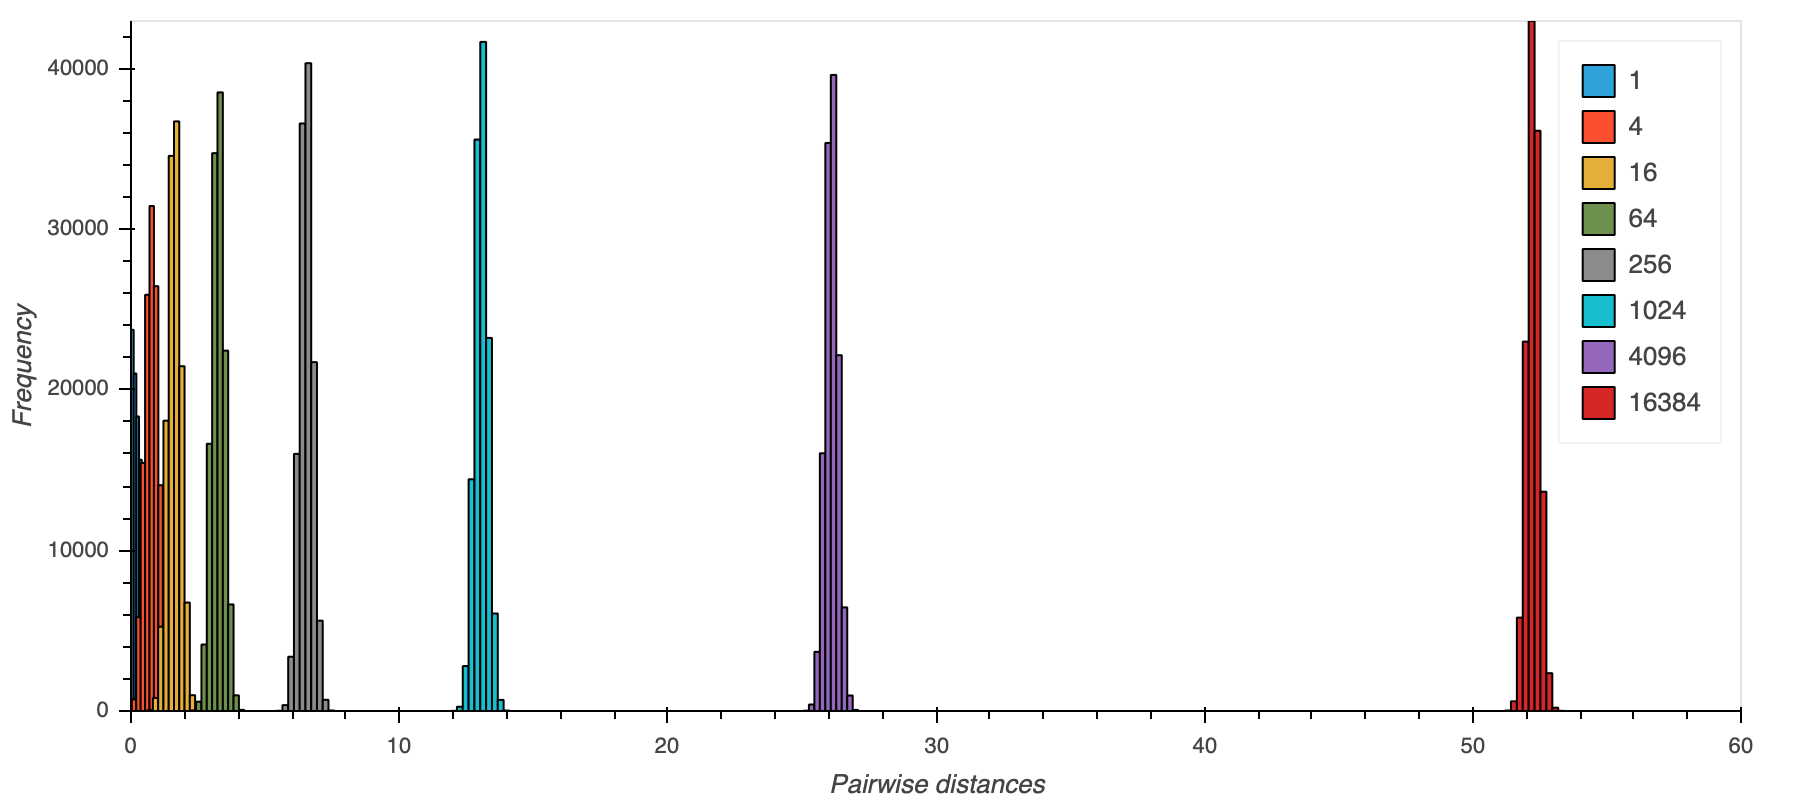
\includegraphics[width=400px, height=178px]{Figures/pairwise_dist}
		%\decoRule
		\caption[Durchsch. Distanz]{Paarweise Distanzen von $N=500$ zuf�llig gleichverteilten Punkten im $R^D$.}
		\label{fig:Curse}
	\end{figure}

	Unter anderem kann man dem \textit{Fluch entfliehen}, in dem die Distanzen mit der Distanz zum ersten Nachbarn normalisiert werden. %TODO: f�ge Grafik ein 
	Dies wenden wir auf unsere erweiterten Metriken $\bar{d}_i$ an und erhalten erweiterte Pseudometriken, 
	
	\begin{align}
		d_i(\mathbf{x}_i,\mathbf{x}_j) \coloneqq \max(0, \bar{d}_i(\mathbf{x}_i,\mathbf{x}_j) - \bar{d}_i(\mathbf{x}_i,\mathbf{x}_{i_1})).
		\label{eq:di}
	\end{align}

	\begin{rem}
		Wir nehmen an, dass unsere Daten $X$ keine Duplikate enthalten. Diese Annahme ist gerechtfertigt, da wir prim�r Aussagen �ber die 
		Beziehung zwischen den Datenpunkten treffen m�chten. Der erste Nachbar ist also ein \textit{echter Nachbar}, mit 
		$\bar{d}_i(\mathbf{x}_i,\mathbf{x}_{i_1}) > 0$. 
	\end{rem}

	\begin{rem}
		F�r den Fall, das die Metrik der zugrundeliegenden Mannigfaltigkeit $d_\M$ bekannt ist, setzen wir in Gleichung (\ref{eq:tilde}) 
		$\tilde{d}_i \coloneqq d_\M$ und wenden die Modifikationen aus Gleichungen (\ref{eq:bar}) und (\ref{eq:di}) an um $d_i$ zu erhalten. 
	\end{rem}

	Die erweiterten Pseudometriken $d_i$ liefern uns lokal die Geod�te, welche hilfreich ist die zugrundeliegende Mannigfaltigkeit zu beschreiben. 
	Allerdings sind die Metriken nicht zwingend miteinander kompatibel. Eine L�sung f�r die Inkompatibilit�t der Metriken werden wir im folgenden Abschnitt beschreiben.

%----------------------------------------------------------------------------------------

\section{Topologische Repr�sentation} \label{sec:repr}
	In Satz \ref{thm:adj} haben wir gesehen, dass es eine Adjunktion zwischen topologischen R�umen und simplizialen Mengen gibt. 
	Wir k�nnten die in Gleichung (\ref{eq:di}) definierten Metriken als topologische R�ume mit $\{(X,\tau_i)\}_{1 \leq i \leq N}$ und 
	der von $d_i$ induzierten Topologie $\tau_i$ auffassen, diese mittels singul�re Mengen Funktors in simpliziale Mengen �berf�hren 
	und die Mengen Vereinigen. Durch diese Konstruktion w�rden uns wichtige Informationen verloren gehen. Um dies zu vermeiden, 
	werden wir eine Adjunktion zwischen der Kategorie der erweiterten pseudo-metrischen R�ume $\EPMet$ und der Kategorie der 
	unscharfen simplizialen Mengen $\sFuzz$ konstruieren.

	\begin{rem}
		Da wir nur endliche Datens�tze betrachten, werden wir uns auf die \textit{Unterkategorien} der endlichen erweiterten pseudo-metrischen R�ume 
		$\fEPMet$ und endlichen unscharfen simpliziale Mengen $\fsFuzz$ beschr�nken. Eine Unterkategorie besteht aus Teilmengen der Objekte und Morphismen 
		der zugeh�rigen Kategorie. 
	\end{rem}

	\begin{defn}
		Der Funktor $\fReal : \fsFuzz \to \fEPMet$ ist gegeben durch

		\begin{align}
			\fReal(X) \coloneqq \varinjlim \fReal(\Delta^n_{<a}),
		\end{align}

		wobei,

		\begin{align}
			 \quad \fReal(\Delta^n_{<a}) &\coloneqq (\{x_1,\dotsc, x_n\}, d_a), \\
			 \quad d_a(x_i,x_j) &\coloneqq \begin{cases}
			 								   0  			&\text{, falls } i = j \\
			 								   -\log(a)		&\text{, sonst.}
			 							  \end{cases}
		\end{align}

		Die Wirkung des Funktors $\fReal$ auf einem Morphismus $\Delta^n_{<a} \to \Delta^m_{<b}$, mit $a \leq b$ und $\sigma: \Delta^n \to \Delta^m$, 
		ist gegeben durch $(\{x_1,\dotsc,x_n\},d_a) \mapsto (\{x_{\sigma(1)},\dotsc,x_{\sigma(n)}\},d_b)$.
	\end{defn}

	% \begin{rem}
	% 	Dabei betrachten wir �hnlich zu Satz \ref{thm:adj} den Limes �ber \dots %TODO
	% \end{rem}

	\begin{rem}
		Der Funktor ist wohldefiniert, da aus $a \leq b, d_a \geq d_b$ folgt. Somit ist die Wirkung von $\fReal$ auf einem Morphismus von $\fsFuzz$ 
		nichtexpansiv und somit ein Morphismus von $\fEPMet$.
	\end{rem}

	\begin{thm}
		Die Funktoren $\fReal$ und $\fSing : \fsFuzz \to \fEPMet$, wobei f�r $Y \in \fEPMet$ gilt,

		\begin{align}
			\fSing(Y) : ([n], [0,a)) \to \hom_\fEPMet (\fReal(\Delta^n_{<a}), Y),
		\end{align}

		sind zueinander adjungiert.
	\end{thm}

	% TODO: Intuition

	\begin{rem}
		Ein Beweis findet sich in \cite{UMAP}. Die wesentliche Idee ist dabei, dass Funktoren welche Limiten erhalten einen rechts adjungierten 
		Funktor besitzen, nach Konstruktion erh�lt $\fReal$ Limiten. Zus�tzlich wird f�r den Beweis das Yoneda Lemma und Gleichung (\ref{eq:colimit}) 
		verwendet. 
	\end{rem}

	Die konstruierte Adjunktion erm�glicht es uns nun die erweiterten pseudo-metrischen R�ume $\{(X,d_i)\}_{1 \leq i \leq N}$, 
	mit $d_i$ aus Gleichung (\ref{eq:di}), mittels des $\fSing$ Funktors als unscharfe simpliziale Mengen darzustellen. 
	Diese verkn�pfen wir mittels t-Conorm und erhalten die \textit{unscharfe topologische Repr�sentation} des Datensatzes $X$

	\begin{align}
		\tConorm \fSing((X, d_i)).
		\label{eq:toprep}
	\end{align}

	%-----------------------------------

	\subsection*{Intuition der Repr�sentation}

	Der folgende Absatz soll die Konstruktion der unscharfen topologischen Repr�sentation intuitiv erkl�ren. Dabei werden wir an einigen Stellen 
	mathematische Strenge gegen eine illustrative Herangehensweise eintauschen.	

	Lokale Eigenschaften der Daten werden dadurch erhalten, dass wir mit Lemma \ref{lem:geod} die Geod�ten auf der $X$ zugrundeliegenden 
	Mannigfaltigkeit bestimmt haben. F�r die erweiterten pseudo-metrischen R�ume, wird dann eine geeignete unscharfe simpliziale Menge konstruiert. 
	In Abschnitt \ref{seq:sSet} haben wir argumentiert, dass es intuitiv oft gen�gt anstelle einer simplizialen Menge einen Simplizialkomplex zu betrachten. 
	Deshalb k�nnen wir uns den Funktor $\fSing$ als \textit{Abbildung} des erweiterten pseudo-metrischen Raumes $X_i$ auf einen unscharfen 
	Simplizialkomplex $\mathcal{K}_i$ vorstellen, wobei jeder Simplex einen Zugeh�rigkeitsgrad hat. 

	Betrachten wir nun das $1$-Skelett von $\mathcal{K}_i$, so sind die $0$-Simplizes die $\mathbf{x}_j \in X$ mit Zugeh�rigkeitsgrad $1$. 
	Die $1$-Simplizes beschreiben Abst�nde zwischen den $\mathbf{x}_j$, wobei der Zugeh�rigkeitsgrad eines $1$-Simplizes aus $\mathcal{K}_i$, mit Facetten 
	$\mathbf{x}_j, \mathbf{x}_l$, gerade $\exp(-d_i(\mathbf{x}_j, \mathbf{x}_l))$ entspricht. Der Zugeh�rigkeitsgrad des ersten Nachbarn von $\mathbf{x}_i$ 
	in $\mathcal{K}_i$ ist also stets $1$ und nimmt f�r weiter entfernte Nachbarn exponentiell ab. Die Repr�sentation erh�lt also metrische Informationen 
	der $\mathbf{x}_i$, bevorzugt dabei allerdings stark die lokalen Abst�nde. Dies spiegelt Aussage des Lemma \ref{lem:geod} wieder, dass wir nur lokal 
	zu $\mathbf{x}_i$ die Geod�te bestimmen k�nnen. 

	Um die lokal unterschiedlichen Zugeh�rigkeitsgrade der $1$-Simplizes % TODO:

	Die Vereinigung der unscharfen simplizialen Mengen in Gleichung (\ref{eq:toprep}) l�sst sich wie folgt f�r den stark vereinfachten Fall des $1$-Skelett 
	der Simplizialkomplexe $\mathcal{K}_i$ beschreiben. Die $0$-Simplizes bleiben unver�ndert. 

	Wir werden sp�ter, in Kapitel \ref{Implementierung}, auf diese Interpretation der $1$-Simplizes zur�ckkommen. 
	Doch zuerst m�chten wir noch beschreiben, wie die unscharfe topologische Repr�sentation f�r das UMAP Verfahren genutzt wird um 
	eine niedrigdimensionale Darstellung der Daten zu finden.

%----------------------------------------------------------------------------------------

\section{Einbettung} \label{sec:einb}
	In diesem Abschnitt soll eine 

	Um die niedrigdimensionale Repr�sentation der hochdimensionalen anzupassen wird f�r das UMAP Verfahren die 
	Kreuzentropie zwischen zwei unscharfen (simplizialen) Mengen vorgeschlagen. 
	
	\begin{equation}
		C((A,\mu), (A, \nu)) \coloneqq \sum_{a \in A} \left(\mu(a)\log\left(\frac{\mu(a)}{\nu(a)}\right) +  \left(1-\mu(a)\right)\log\left(\frac{1-\mu(a)}{1-\nu(a)}\right)  \right)
		\label{eq:crossentropy}
	\end{equation}
	
	In Abschnitt \ref{seq:numerische_formulierung} werden wir die Kreuzentropie genauer betrachten.

%----------------------------------------------------------------------------------------

% Zeitplan:
% Sa: Kapitel 2,3,4 vervollst�ndigen, Einleitun und Appendix schreiben
% So: Plots plots plots, �berarbeiten 



 
%!TEX root = ../main.tex

\chapter{Implementierung} 

\label{Implementierung}

% Docs for algorithms: 
% http://mirror.physik-pool.tu-berlin.de/pub/CTAN/macros/latex/contrib/algorithmicx/algorithmicx.pdf

%----------------------------------------------------------------------------------------

% \newcommand{\indexij}[1][v]{{#1}_{ij}}  % Symbol for v_{ij}
\newcommand{\vij}{v_{ij}}  % Symbol for b_{ij}
\newcommand{\wij}{w_{ij}}  % Symbol for w_{ij}

%----------------------------------------------------------------------------------------
%----------------------------------------------------------------------------------------

% TODO: Beschreibung der L�cke in diesem Kapitel oder in UMAP
% \section{Einleitung}
In diesem Kapitel m�chten wir die Implementierung des UMAP Verfahren beschreiben. 
Die vollst�ndige Berechnung aller Simplizes hat eine exponentielle Laufzeit, da hierf�r 
alle Teilmengen unseres $N$-elementigen Datensatzes betrachtet werden m�ssten. 
In der Implementierung von McInnes et. al. \cite{cpu}  werden hingegen nur alle 
zweielementigen Teilmengen betrachtet. 
Wie wir in Kapitel \ref{Experimente} sehen werden, liefert uns diese Approximation des 
\cech-Komplexes sehr gute visuelle Ergebnisse.  % Cech Komplex?
Zuerst werden wir den Algorithmus mit seinen Subroutinen in Pseudo-Code angeben. Danach 
werden wir Ans�tze nennen um die L�cke zwischen Theorie und Praxis zu schlie�en. 
Zus�tzlich werden wir die rechenintensiven Schritte des Verfahrens betrachten und eine 
effizientere Implementierung auf der GPU betrachten.

%----------------------------------------------------------------------------------------

% N O T I Z E N
% Cite Numba 24
% Plot wie die stetige Approximierung f�r verschiedene Parameter a und b aussieht.

% T E X T B A U S T E I N E
% 

%----------------------------------------------------------------------------------------
%----------------------------------------------------------------------------------------

\section{Pseudo-Code}
   Das berechnen des 

   \begin{algorithm}
   \caption{UMAP Algorithmus}
   \label{algorithm:umap}
   \begin{algorithmic}[1]
   \Function{UMAP}{$X, N, D, d, min\_dist, n\_epochs$}  %description
      \For{$x \in X$}
         \State $knn(x) \gets k\text{-n�chste-Nachbarn}(x)$ \label{alg:kNN}
         \State $graph(x) \gets \bot_{y \in knn(x)} (\{x, y\}, exp(-d_{x,y})) \ \bot \ \bot_{y \in X \setminus \{x\}} (\{x, y\}, 0)$ \label{alg:graph}
      \EndFor
      \State $V \gets \text{gewichtete Adjazenzmatrix}(\bigcup_{x \in X} graph(x))$
      \State $D \gets \text{Grad-Matrix des Graphen } V$ \label{alg:grad}
      \State $L \gets D^{1/2} (D-V) D^{1/2}$ \Comment{Symmetrische normalisierte Laplace-Matrix}
      \State $evec \gets \text{sortierte Eigenvektoren von } L$
      \State $Y \gets evec[1,\dots,d\text{+}1]$ \label{alg:spec}
      \State $Y \gets OptimizeEmbedding(Y, min\_dist, n\_epochs)$
      \State \textbf{return} $Y$
   \EndFunction
   \end{algorithmic}
   \end{algorithm}

   In Abschnitt \ref{seq:kNN} werden zwei effiziente Verfahren f�r die k-n�chste-Nachbarn Suche (Zeile \ref{alg:kNN}) angeben. 
   
   % TODO: Referenzen einf�gen
   Der in Zeile \ref{alg:graph} verwendete $\bot$ Operator verdeutlicht, dass wir die Kantengewichte mittels wahrscheinlichkeitstheoretischer 
   t-Conorm vereinigen. 
   In den von uns verwendeten Implementierung des UMAP Verfahrens \cite{cpu,GPUUMAP} wird ein zus�tzlicher Hyperparameter verwendet, welcher 
   eine Verallgemeinerung der Vereinigung darstellt (siehe:). %TODO: Verweis auf set_op_mix_ratio
   Zus�tzlich ist zu beachten, dass die Vereinigung in Zeile \ref{alg:graph} ungerichtete Kanten betrachtet. Der so erhaltene ungerichtete Graph 
   besitzt aufgrund der Symmetrie der t-Conorm wohldefinierte Kantengewichte.

   Die Grad-Matrix $D$ (Zeile \ref{alg:grad}) ist eine Diagonalmatrix, wobei  $d_{ii} \coloneqq  \sum_{1 \leq k \leq N} a_{ik}, (1 \leq i \leq N)$. 
   F�r den Spezialfall, der ungewichteten Adjazenzmatrix, beschreibt $d_{ii}$ also den Grad des Knoten $i$. 

   Die Initialisierung der niedrigdimensionalen Repr�sentation $Y$ in Zeile \ref{alg:spec} ist die spektrale Einbettung des Graphen. 
   referenziere seqution oder beschreibe die Sinnhaftigkeit hier % TODO: seqution?


   Um eine Unterscheidung zwischen der theoretischen Sichtweise auf das UMAP Verfahren, welche alle $k$-Simplizes 
   $(1 \leq k \leq N)$ ber�cksichtigt, und der praktischen Implementierung zu verdeutlichen werden wir die 
   verwendete Notation anpassen. 
   % TODO: F�ge Referenzen zu UMAP ein.
   Die allgemeine Kreuzentropie f�r unsichere Mengen ref{} l�sst sich f�r den Fall, dass nur das 1-Skelett betrachtet 
   wird wie folgt notieren:

   \begin{alignat}{2}
      C &= \sum_{1 \leq i,j \leq N} \vij \log\left(\frac{\vij}{\wij}\right) + (1-\vij) \log\left(\frac{1-\vij}{1-\wij}\right) \\
        &= 
          \begin{aligned}[t]
            &  \sum_{1 \leq i,j \leq N} (\vij \log(\vij) + (1-\vij) \log(1-\vij)) \\
            &- \sum_{1 \leq i,j \leq N} (\vij \log(\wij) - \sum_{1 \leq i,j \leq N} (1-\vij) \log(1-\wij))
         \end{aligned} \\
       &=  C_v - \sum_{1 \leq i,j \leq N} (\vij \log(\wij) - \sum_{1 \leq i,j \leq N} (1-\vij) \log(1-\wij))
   \end{alignat}

   , wobei $\vij = \mu(a), \wij = \nu(a), \vij \in V, a \in A \text{ s.d. } a $ ist 1-Simplex zwischen den Datenpunkten $i, j$. 


%----------------------------------------------------------------------------------------

\section{Spektrale Einbettung}
   Der Laplace Operator ist eine diskrete Approximation des Laplce-Beltrami Operators. Spectrale Eeinbettung \dots

%----------------------------------------------------------------------------------------

\section{Profiling}
   In Kapitel \ref{Experimente} werden wir genauer auf die tats�chliche Laufzeit des UMAP Algorithmus eingehen. 
   An dieser Stelle m�chten wir die rechenintensiven Subroutinen des Verfahrens ausmachen. Daf�r haben wir den 
   Python cProfiler verwendet, dieser misst die Laufzeit der aufgerufenen Funktionen. 
   Um f�r verschiedene Umgebungsdimensionen vergleichbare Ergebnisse zu erhalten, haben wir $N = \num{10000}$ 
   Datenpunkte in $10$ unterschiedlichen $D = [100, 500, 1000, 5000, 10000, 50000]$-dimensionalen Gau�-verteilten 
   Datenwolken gew�hlt. F�r den Funktionsaufruf haben wir die Standardparameter verwendet, insbesondere haben wir 
   die Daten in einen zweidimensionalen Raum eingebettet.
   Dabei ist uns aufgefallen, dass besonders der k-n�chste-Nachbarn-Algorithmus und die Optimierung mittels 
   stochastischem Gradienten Verfahren einen gro�en Teil der Laufzeit des Verfahrens beanspruchen. In Tabelle 
   \ref{table:profiling} sind die Ergebnisse der Profilierung zusammengefasst. 

   \begin{table}
   \begin{tabular}{l|ll}
   D     & Laufzeit NN-Descent & Laufzeit der Optimierung \\ \hline
   100   & 9\%                 & 75,3\%                   \\
   500   & 12\%                & 73,8\%                   \\
   1000  & 14\%                & 72,9\%                   \\
   5000  & 30,4\%              & 58\%                     \\
   10000 & 44\%                & 45,1\%                   \\
   50000 & 78,8\%              & 14,8\%                  
   \end{tabular}
   \caption{$D$ beschreibt die Gr��e der Umgebungsdimension. Abh�ngig von D haben wir die Laufzeit des UMAP Verfahrens 
            profiliert. Die zweite und dritte Spalte beziehen sich auf die relativen Laufzeiten des kNN Verfahrens und 
            der Optimierung der Einbettung.}
   \label{table:profiling}
   \end{table}

   Insbesondere scheint der \textit{NN-Descent} Algorithmus \cite{k-NNG} die Laufzeit des UMAP Verfahren f�r 
   hochdimensionale Daten stark zu beeinflussen. 
   Wir werden beide rechenintensiven Subroutinen im folgenden betrachten und geeignete Verbesserungen diskutieren. 

%----------------------------------------------------------------------------------------

\section{Gradienten Verfahren} \label{seq:SGD}
   Um die Zielfunktion zu o{}ptimieren wird im UMAP Verfahren ein stochastisches Gradienten Verfahren (kurz: \textit{SGD}) 
   genutzt. 
   In \cite{SGDGPU} werden verschiedene Implementierungen verglichen.

%----------------------------------------------------------------------------------------

\section{N�chste-Nachbarn-Klassifikation} \label{seq:kNN}
% Einer der beiden rechenintensivsten Subroutinen im UMAP Algorithmus ist die n�chste Nachbar suche.
% in \cite{Tang} (k-NN is bottleneck) werden 3 verschiedene Methoden verglichen. Sehr effizient ist auch die 
% Facebook FAISS Methode.
   Zum effizienten finden der 1-Simplizes der topologischen Repr�sentation unserer Daten, ben�tigen wir einen 
   k-n�chste-Nachbarn-Algorithmus (kurz: \textit{kNN-Algorithmus}). 
   %TODO: Beschreibung was ein kNN-Alg macht

   Das Ergebnis eines kNN-Algorithmus wird meist in einem ungerichteten Graph -- dem kNN-Graph -- dargestellt, 
   wobei die Knoten den Datenpunkten entsprechen und die Kanten den Nachbarschaftsbeziehungen, 
   somit besitzt jeder Knoten Grad k.

   Bei einer naiven Implementierung betr�gt die Laufzeit $\mathcal{O}(N^2D)$ (wobei N die Anzahl der Datenpunkte  % TODO: warum N^2D?
   und D die Dimension der Datenpunkte ist). Mit einer effizienten Implementierung ist in der Praxis eine 
   ann�hernd in N lineare Laufzeit m�glich. Die Herangehensweisen lassen sich nach \cite{Tang} in drei Kategorien 
   einteilen. (1) Baum basierte Verfahren auf Partitionen des Raumes, (2) Hashfunktionen auf lokalen Teilgebieten des Raumes 
   (3) Nachbarschafts-Erkundungen. 

   Wir m�chten nun zwei Verfahren vorstellen. 
   \subsection*{NN-Descent}
      Der NN-Descent Algorithmus \cite{k-NNG} beruht auf dem Prinzip der Nachbarschafts-Erkundungen. Dabei wird ein 
      initialer kNN-Graph iterativ verbessert, unter der Annahme, dass die Nachbarschaftsbeziehung 
      transitiv ist, f�r zwei vorhandene Nachbarschaftspaare $(x, y), (y,z)$ also mit hoher Wahrscheinlichkeit auch 
      ein Nachbarschaftspaar $(x,z)$ im kNN-Graph existiert. 
      Der initiale Graph im NN-Descent Verfahren wird dabei zuf�llig gew�hlt. Dies kann dazu f�hren, dass nur 
      lokal optimale k-NN-Graphen gefunden werden. Dies k�nnte laut \cite{EFANNA} dadurch verbessert werden, indem 
      f�r die Initialisierung \enquote{random projection trees}, wie in \cite{Tang}, verwendet werden. 

      Ein Vorteil des NN-Descent Verfahren ist, dass kein globaler Index der verwaltet werden muss. Somit ist eine 
      Anwendung auf gro�en Datens�tzen m�glich welche nicht komplett in den Arbeitsspeicher (RAM) des verwendeten Rechners 
      geladen werden k�nnen. 

      Nachteil des NN-Descent Algorithmus ist die Speicherplatzkomplexit�t, diese ist durch $\mathcal{O}(N^2)$ beschr�nkt. 
      Im wesentlichen ist dies dadurch begr�ndet, dass paarweise die �hnlichkeit, welche im Falle von UMAP durch die Metrik 
      des Umgebungsraums gegeben ist, gespeichert wird. Aufgrund dessen, dass nur lokale Optima garantiert sind, ist das Ergebnis 
      des NN-Descent Verfahren approximativ. In \cite{UMAP} wird jedoch argumentiert, dass dies wegen des Informationsverlust 
      bei Dimensionsreduktionen kaum Auswirkungen auf die resultierende Einbettung hat. 


   \subsection*{FAISS}
      Das FAISS Bibliothek \cite{FAISS} nutzt die Architektur einer GPU aus. Dabei baut FAISS eine effiziente Datenstruktur, 
      welche f�r die Vektoren die n�chsten Nachbarn speichert. Somit ist eine sehr schnelle Implementierung 
      f�r das aufstellen des k-NN-Graphen m�glich. 

      Der RAM der meisten GPUs ist stark begrenzt. Um dennoch mit gro�en Datens�tzen zu arbeiten werden komprimierte 
      Darstellungen der Vektoren genutzt. % TODO: Referenzen einf�gen, aus FAISS
      F�r FAISS werden \enquote{product quantization codes} genutzt. % TODO: referenz und kurze Beschreibung 

      Vorteile der FAISS Datenstruktur sind die effiziente Implementierung auf GPUs und das sowohl exakte Ergebnisse 
      sowie Approximationen f�r die n�chsten Nachbarn angegeben werden k�nnen. Die R�ckgabe approximativer 
      Ergebnisse erh�lt Laufzeit sowie Speicherplatz Vorteile. 

      Nachteil des FAISS Verfahren ist, dass zurzeit nur die euklidische Distanz unterst�tzt wird. 






%!TEX root = ../main.tex

\chapter{Experimente} \label{Experimente}

%----------------------------------------------------------------------------------------

% A U F B A U
	% Welche Verfahren
	% Welche Daten
	% Welche Ergebnisse unter welchen Parametern
	% Welche Laufzeit
	% Welche Schlussfolgerungen

	% N O T I Z E N
	% Cartoonset, MNIST, (WIND)
	% PCA, UMAP, t-SNE, LargeVis

	% Test transform function

	% Google News f�r n_samples Dimension

	% Outlier, add completly different images 

	% Erw�hne analytische Bewertungen der Einbettungen
	% trustworthiness-continuity (Kaski et al., 2003)
	% mean (smoothed) precision-recall (Venna et al., 2010)
	% nearest-neighbor accuracy (Van Der Maaten et al., 2009)

	% Stabilit�t der Ergebnisse

	% Komplett neue Gesichter

	% Cluster on FMNIST, Scores on MNIST (Costfunction and SVD)

	% Auswirkung von sampling auf kleinen Datens�tzen

	% T E X T B A U S T E I N E
	% 'Empirisches testen der Hypothesen/ Annahmen'
	% 'UMAP auf realen/echten Daten'
	% In \cite{UMAP} wurde bereits die Stabilit�t des Verfahrens getestet.
	% Insbesondere verweisen wir auf Abbildung 3,4 in Abschnitt 5.
	% Die Stabilit�t des UMAP Verfahrens ist 

	% Mehr Datenpunkte, dann h�here perplexit�t f�r gleichen Ausgang, �hnlich zu n_neighbor
	% tSNE vergr��ert Regionen mit h�herer Dichte

	% Bei cartoonpca784 bleibt 99,842% der Varianz erhalten.
	% Bei cartoonpca10k weniger als 10^-5 * 2 verlust der Varianz 

	% Um eine gute Interpretation der Daten zu geben ist es wichtig ein sehr gutes Verst�ndnis 
	% der Datens�tze zu besitzen, deshalb haben wir uns auf leicht interpretierbare Daten beschr�nkt

	% Verweise auf Daten und erw�hne deutlich feinere Struktur von UMAP
	% https://www.biorxiv.org/content/biorxiv/early/2018/04/10/298430.full.pdf

	% Keine Wordembeddings, da die Vorvererbeitung sehr wichtig ist.

%----------------------------------------------------------------------------------------
%----------------------------------------------------------------------------------------

% \section{Einleitung}
	Nach ausf�hrlicher Darstellung der Theorie des UMAP Verfahrens, m�chten wir nun UMAP auf 
	drei Datens�tzen mit alternativen Verfahren empirisch testen.
	Wir werden eine m�glichst vollst�ndige Darstellung der Ergebnisse in dieser Arbeit pr�sentieren. 
	Allerdings ist es zu empfehlen die Ergebnisse in einem interaktiven Jupyter notebook zu betrachten. 
	Dieses befindet sich auf der beigelegten CD oder auf GitHub
	\footnote{\url{https://github.com/reinerschristopher/review_DR_algorithms}}. 
 	
 	In diesem Kapitel werden wir in Abschnitt \ref{sec:verfahren} zwei alternative Verfahren beschreiben.
 	Wir werden in Abschnitt \ref{sec:bwertung} beschreiben, wie wir die Einbettungen bewertet haben. 
 	Abschnitt \ref{sec:cartoonset} wird einen neuen Datensatz, das Cartoon Set vorstellen. Dieses besitzt eine 
 	komplexere Struktur und bietet uns somit mehr Raum f�r eine Analyse der Einbettungen.
 	In Abschnitt \ref{sec:FMNIST} werden wir die Einbettungen verschiedener Verfahren auf dem bekannten 
 	MNIST Datensatz betrachten. Dieses Kapitel werden wir mit der Betrachtung der Laufzeiten abschlie�en. 

%----------------------------------------------------------------------------------------

\section{Alternative Verfahren} \label{sec:verfahren}
	Wir haben uns dazu entschieden UMAP mit t-SNE, TriMap und PCA zu vergleichen. Die ersten beiden 
	Verfahren sollen kurz eingef�hrt werden, wobei wir insbesondere die wichtigen Hyperparameter der 
	Verfahren angeben. Eine Kenntnis des PCA Verfahrens setzen wir voraus. 
	An dieser Stelle ist zu bemerken, dass in den letzten Jahren zahlreiche neue DR Verfahren entwickelt wurden. 
	Aufgrund dessen k�nnen wir in dieser Arbeit nur eine kleine Teilmenge der DR Verfahren betrachten. 
	Ein sehr ausf�hrlicher Vergleich findet sich in \cite{Maaten2008}. %, dieser ber�cksichtigt allerdings keine neueren Verfahren, da er 2008 publiziert wurde. 


	Da die Implementierungen des Laplacian Eigenmaps Verfahrens und Isomap Verfahrens schlecht f�r gro�e 
	Datens�tze skalieren, haben wir uns bewusst dazu entschieden, diese nicht mit in die Analyse aufzunehmen. 

	%-----------------------------------

	\subsection{t-SNE}
	% TODO: wichtige Terme einf�gen?
	Das t-SNE Verfahren \cite{tSNE} ist zur Zeit eines der bekanntesten und meistgenutzten 
	nicht-linearen Dimensionsreduktionsverfahren. Dabei wird t-SNE fast ausschlie�lich 
	zur Visualisierung genutzt, da die Laufzeit f�r h�here Einbettungsdimensionen schlecht ist. 
	% TODO: Wie wir sp�ter sehen werden. (oder unten?)

	t-SNE konstruiert zuerst eine Wahrscheinlichkeitsverteilung $P$ auf Paaren $(i, j)$ der hochdimensionalen 
	Datenpunkten. Diese ist so gew�hlt, dass Paare �hnlicher Objekte eine h�here Wahrscheinlichkeit 
	zugeordnet bekommen, wohingegen sehr unterschiedliche Datenpunkte eine Wahrscheinlichkeit nahe $0$ haben. 
	Die �hnlichkeit der Punkte wird dabei meist mittels der euklidischen Distanz gemessen, 
	kann aber �hnlich wie im UMAP Algorithmus durch andere Metriken ersetzt werden. Um $P$ zu konstruieren 
	wird eine Gau�verteilung genutzt, wobei die Varianz abh�ngig vom \code{perplexity} Parameter ist. 
	Die so erhaltenen Wahrscheinlichkeiten $p_{i | j}$ sind im Allgemeinen nicht symmetrisch. 
	Die Symmetrie wird durch mitteln der Daten erhalten. 

	�hnlich wird eine Wahrscheinlichkeitsverteilung $Q$ im niedrigdimensionalen Raum mithilfe der 
	studentschen t-Verteilung konstruiert. Urspr�nglich wurde $Q$ ebenfalls durch eine Gausverteilung 
	konstruiert, das so erhaltene Verfahren (SNE \cite{tSNEvar1}) ist allerdings aufgrund einer 
	schwierig zu optimierenden Zielfunktion und dem \enquote{crowding problem} wenig praktikabel.

	Um die d-dimensionale Repr�sentation der Daten zu optimieren wir die Kullback-Leiber Divergenz 
	von zwischen $P$ und $Q$ bez�glich der $y_i$ minimiert. % TODO: werden y_i in Einleitung erw�hnt?

	Seit der Ver�ffentlichung des Verfahrens wurden zahlreiche Verbesserungen, 
	insbesondere f�r die Laufzeit, vorgeschlagen \cite{tSNEmod1,tSNEmod3}. 
	Dabei ist besonders Barnes-Hut-SNE \cite{tSNEmod2} zu erw�hnen, allerdings sollte hier beachtet werden, 
	dass aufgrund der Konstruktion einer speziellen Datenstruktur die Laufzeit f�r $d>3$ sehr schlecht ist.

	Die von t-SNE produzierte Repr�sentation der Daten ist vom \code{perplexity} Parameter abh�ngig. 
	Dabei kann man festhalten, je gr��er die \code{perplexity} ist, desto gr��er ist die Varianz  % TODO: Verweise auf die Gleichungen oben 
	des Gau�verteilung. Somit werden f�r gro�e \code{perplexity} Werte globalere Strukturen erfasst, 
	da der Gau�kern sehr breit ist. Wenn der \code{perplexity} Parameter in der Gr��enordnung der 
	Anzahl an Datenpunkten $N$ liegt gleicht t-SNE dem MDS Verfahren. % TODO: Referenz? 

	Der zweite wichtige Hyperparameter, welchen wir beschreiben m�chten ist die \code{exaggeration}.
	meistens wird hier zwischen \code{early-} und \code{late-exaggeration} unterschieden. 
	Im wesentlichen verbessert der Parameter die Optimierung des Gradienten und sorgt daf�r, 
	dass Punkte desselben Clusters m�glichst schnell in der niedrigdimensionalen Repr�sentation 
	gruppiert werden \cite{tSNEcluster}. Der \code{late-exaggeration} wie in \cite{tSNEmod3} 
	beschrieben kontrahiert gefundene Cluster, so lassen sich in einer 2- oder 3-dimensionalen 
	Darstellung leichter Cluster bestimmen - entweder visuell oder mittels Clustering-Verfahren. 

	Wir werden reale Datens�tze analysieren und das Verhalten der Hyperparameter beschreiben, um 
	ein zus�tzliches Verst�ndnis f�r die von t-SNE genutzten Hyperparameter zu bekommen 
	empfiehlt sich \cite{tSNEparam}, dort werden interaktiv auf k�nstlich erzeugten Datens�tzen 
	die Auswirkung der Parameter gezeigt.

	F�r unsere Experimente haben wir die scikit Implementierung des t-SNE Verfahren genutzt \cite{scikit-learn}.
	Zus�tzlich haben wir die openTSNE \cite{opentSNE} Implementierung genutzt. Diese beschleunigt 
	die Laufzeit des t-SNE Algorithmus durch eine zus�tzliche Fouriertransformation \cite{tSNEmod3}.
	Die openTSNE Implementierung besitzt im Vergleich zur scikit Implementierung die M�glichkeit 
	den \code{late-exaggeration} Parameter zu spezifizieren. % TODO: sp�ter sehen wir die 

	Um einen Laufzeitvergleich mit der GPU Implementierung des UMAP Verfahrens zu erm�glichen, 
	werden wir eine GPU Implementierung von t-SNE betrachten \cite{tSNEGPUcode}. 
	Eine Beschreibung findet sich in \cite{tSNEGPUpaper}.

	%-----------------------------------

	\subsection{TriMap}
	Das TriMap Verfahren \cite{TriMap} soll eine globalere Repr�sentation der Daten finden als 
	beispielsweise t-SNE, da nicht nur paarweise die �hnlichkeit zweier Objekte $i, j$ betrachtet wird, 
	sondern stets Triple $i, j, k$. Die so erhaltene globale Struktur der Daten soll die 
	Cluster-Abst�nde der Daten repr�sentieren. Die von uns gew�hlte Implementierung des Verfahrens findet 
	sich in \cite{trimapcode}.

	% TODO: TriMap besser beschreiben. 

	Wir haben diesem Algorithmus gew�hlt, da die Tripletts �hnlichkeiten mit 2-Simplizes des UMAP Verfahren haben.
	Die Tripletts sind vergleichbar mit den 2-Simplizes des UMAP Verfahrens. 
	Insbesondere k�nnen die Ans�tze eine lineare Teilmenge ($O(N)$) an Tripletts zu finden 
	weitere Entwicklungen des UMAP Verfahren motivieren.

%----------------------------------------------------------------------------------------

\section{Bewertung der Ergebnisse} \label{sec:bwertung}
	Um die lokale Qualit�t der Algorithmen zu analysieren haben wir uns die \textit{Cluster} in der 
	$2$-dimensionalen Repr�sentation angeschaut, wobei wir als Cluster eine Teilmenge der Daten bezeichnen, 
	welche deutlich von den anderen Datenpunkten getrennt ist. % TODO: 'Stetigkeit' innerhalb der Cluster?
	Insbesondere bei der Analyse des Cartoon Set \ref{sec:cartoonset} konnten wir gut lokale Strukturen 
	erkennen, da jeder Datenpunkt mehrere Eigenschaften gegeben hat -- im Vergleich zum MNIST und FMNIST 
	Datensatz, wo uns nur ein \textit{Label} pro Datenpunkt gegeben ist. 

	Die globale Struktur der Repr�sentation qualitativ zu bewerten ist subjektiv. Dabei ist insbesondere 
	die Frage -- \enquote{Wie \textit{stark} unterscheiden sich die Cluster?} -- zu beantworten. 

	F�r die qualitative Analyse wird die F�higkeit des Gehirns genutzt Strukturen zu erkennen. 
	Nachteile der qualitativen Analyse sind, (1) die Subjektivit�t und somit Abh�ngigkeit vom Betrachter, 
	(2) dass sie nur im $d$-dimensionalen $(d \leq 3)$ m�glich ist. 
	% und (3) die Problematik, dass es (noch) keine mathematische Formulierung der Bewertung gibt.

	Wir verweisen den Leser auf \cite{Harmeling,Lee2009,Rieck2015} f�r verschiedene Ans�tze 
	DR Verfahren auf eine quantitative Weise zu bewerten.

	In den folgenden Experimenten haben wir uns auf eine qualitative Analyse der Daten beschr�nkt.


%----------------------------------------------------------------------------------------

\section{Cartoon Set} \label{sec:cartoonset}
	In diesem Abschnitt werden wir den \textit{Cartoon Set} Datensatz analysieren \cite{cartoon}. 
	Dabei werden wir,
	\begin{itemize}
		\item die Einbettungen von UMAP mit denen von t-SNE und TriMap visuell bewerten,
		\item und die drei Verfahren auf globale und lokale Strukturen vergleichen, 
		\item an einigen Stellen verdeutlichen wie schwierig die Bewertung der Qualit�t der Einbettung ist.
	\end{itemize}

	%-----------------------------------

	\subsection*{Beschreibung des Datensatzes}
	Der Cartoon Datensatz enth�lt \num{100000} unterschiedliche Bilder von gezeichneten Gesichtern 
	(siehe Abbildung \ref{fig:Cartoon_Sample}). 

	\begin{figure}
		%\centering
		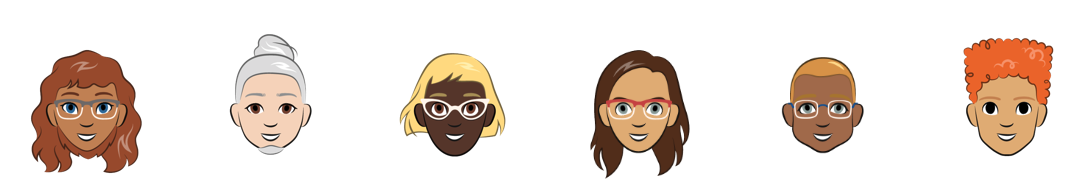
\includegraphics[width=400px, height=73px]{Figures/Cartoon_Sample}
		%\decoRule
		\caption[Ausschnitt des Cartoon Set]{Sechs zuf�llig gew�hlte Gesichter des Cartoon Set.}
		\label{fig:Cartoon_Sample}
	\end{figure}

	Die Bilder wurden aus 16 Labels zusammengesetzt (u.a. Gesichtsform, Gesichtsfarbe, Frisur, Haarfarbe), 
	dabei variiert die Anzahl der M�glichkeiten pro Label zwischen zwei (Augenlid, Wimpern,\dots) und 
	111 (Anzahl m�gliche Frisuren). Die Farben der Komponenten wurden aus einem diskreten RGB Raum gew�hlt. 
	Insgesamt ergibt sich eine m�gliche Anzahl von $10^{13}$ Gesichtern. F�r die Analyse haben wir verschiedene 
	Eigenschaften zusammengefasst um einen besseren �berblick zu haben. 
	Beispielsweise haben wir die 111 Frisuren, nach qualitativer Analyse, zu 19 Frisurformen zusammengefasst. 

	Die urspr�ngliche Gr��e eines Bildes betrug $500 \times 500$ Pixel mit vier Farbkan�len 
	(CYMK-Darstellung der Farben). Aufgrund des gro�en Randes haben wir uns dazu entschieden die Gr��e der 
	Bilder auf $300 \times 300$ ohne nennenswerten Informationsverlust zu verringern. Somit betr�gt die Dimension 
	des Cartoon Set $D = \num{360000}$ und die Anzahl an Beispielen $N$ variiert zwischen $\num{10000}$ und $\num{100000}$. 
	An dieser Stelle ist die sehr hohe Umgebungsdimension hervorzuheben. Typischerweise werden Daten mit einer 
	Umgebungsdimension $D > \num{10000}$ mit PCA auf eine Dimension in den Bereich $D' \in [100,1000]$ vorverarbeitet. 
	Sp�ter werden wir sehen, dass diese Vorverarbeitung bezogen auf unsere Bilddaten keine gro�en Nachteile birgt.  

	Wir haben uns f�r diesen Datensatz entschieden um UMAP auf Daten mit einer komplexeren Struktur zu testen 
	als dies in \cite{UMAP} gemacht wird. Dabei ist auch zu beachten, dass aufgrund der 16 Labels aus 
	welchen die Gesichter bestehen, die Qualit�t einer Einbettung schwieriger zu beurteilen ist als beispielsweise 
	im MNIST Datensatz (siehe Abschnitt \ref{sec:FMNIST}). Wir haben die Bewertung der Einbettung unter der Annahme 
	gemacht, dass \textit{�hnliche} Gesichter \textit{�hnliche} Hautfarben, Frisuren, Haarfarben, Brillen und B�rte 
	besitzen. Diese f�nf Eigenschaften m�chten wir besonders hervorheben, da sie die dominantesten Merkmale des Gesichts 
	beschreiben. Somit werden wir eine Einbettung des Cartoon Set als \textit{gut} bewerten, wenn sie zwischen 
	diesen f�nf Merkmalen unterscheidet.

	% Histogram �ber Verteilung der Frisuren

	% unterschiedliche n_components (range(15))

	% gute ergebnisse wegen aaprox kNN und lokaler Zusammenhang

	% Erw�hne hohe Umbegungsdimension

	%-----------------------------------

	% Globale Struktur sehr gut erhalten und lokale auch, wenig abh�ngig von Parametern
	\subsection*{Qualitative Analyse der Ergebnisse}
	Wir werden nun die Einbettungen bewerten. 
	F�r die Einbettung des Cartoon Set haben wir die voreingestellten Hyperparameter gew�hlt. F�r das UMAP Verfahren haben wir nur den Parameter $\code{n\_neighbors}=50$ 
	und f�r t-SNE den Parameter $\code{perplexity}=40$ gew�hlt, kleinere Parameter der Wert haben Einbettungen mit zu vielen Clustern ergeben. 
	Abbildung \ref{fig:pca_cartoon} zeigt eine Einbettung des Cartoon Set mittels PCA. Dies dient als Startwert unserer Analyse. 
	Im linken Plot sind dabei zwei Linien eingezeichnet. Diese verdeutlichen, dass mittels PCA die Gesichter in 3 Klassen eingeteilt werden k�nnen. 
	Die Farben des Punkte in diesem Plot stellen die Frisurtypen dar. 
	Die oberen blauen und roten Punkte stellen Gesichter mit wenigen Haaren dar, die Punkte eingeschlossen von den beiden Linien stellen Gesichter 
	mit mittellangen und die unteren Punkte Gesichter mit langen Haaren dar. Ebenfalls in Abbildung \ref{fig:pca_cartoon} sind exemplarisch einige 
	Gesichter mit ihrer zugeh�rigen Lage in der Einbettung zu sehen. Der mittlere Plot visualisiert die Gleiche Einbettung, es wurden nur andere labels 
	f�r die Daten genutzt. Die Farben repr�sentieren die Gesichtsfarben, dabei entspricht gelb hellen Hauttypen, lila sehr dunklen und t�rkis/gr�n den restlichen 
	Hauttypen. �hnlich werden im rechten Plot die Farben der Punkte entsprechend ihrer Haarfarben gew�hlt, wobei der Verlauf von gelb �ber gr�n nach lila den Verlauf 
	schwarzen �ber braunen nach blonden/grauen Haarfarben entspricht. Wir werden diese Farbwahl in den anderen Plots beibehalten. Auch hier ist eine Struktur zu 
	erkennen, auff�llig ist dabei, dass die linearen Strukturen vom oberen Drittel schlechter sind als die im unteren Drittel. Dies k�nnen wir dadurch erkl�ren, 
	dass sich l�ngere Haartypen leichter unterscheiden lassen als beispielsweise die Unterscheidung zwischen keinen und sehr wenig kurzen Haaren. 
	Wir k�nnen an dieser Stelle unsere Annahme best�tigen, dass das Cartoon Set eine zugrundeliegende Struktur besitzt, welche unsere Intuition widerspiegelt. 

	\begin{figure} % PCA als Startwert, global sind hair, face_color und hair_color, nicht faicial_hair und glasses
		%\centering
		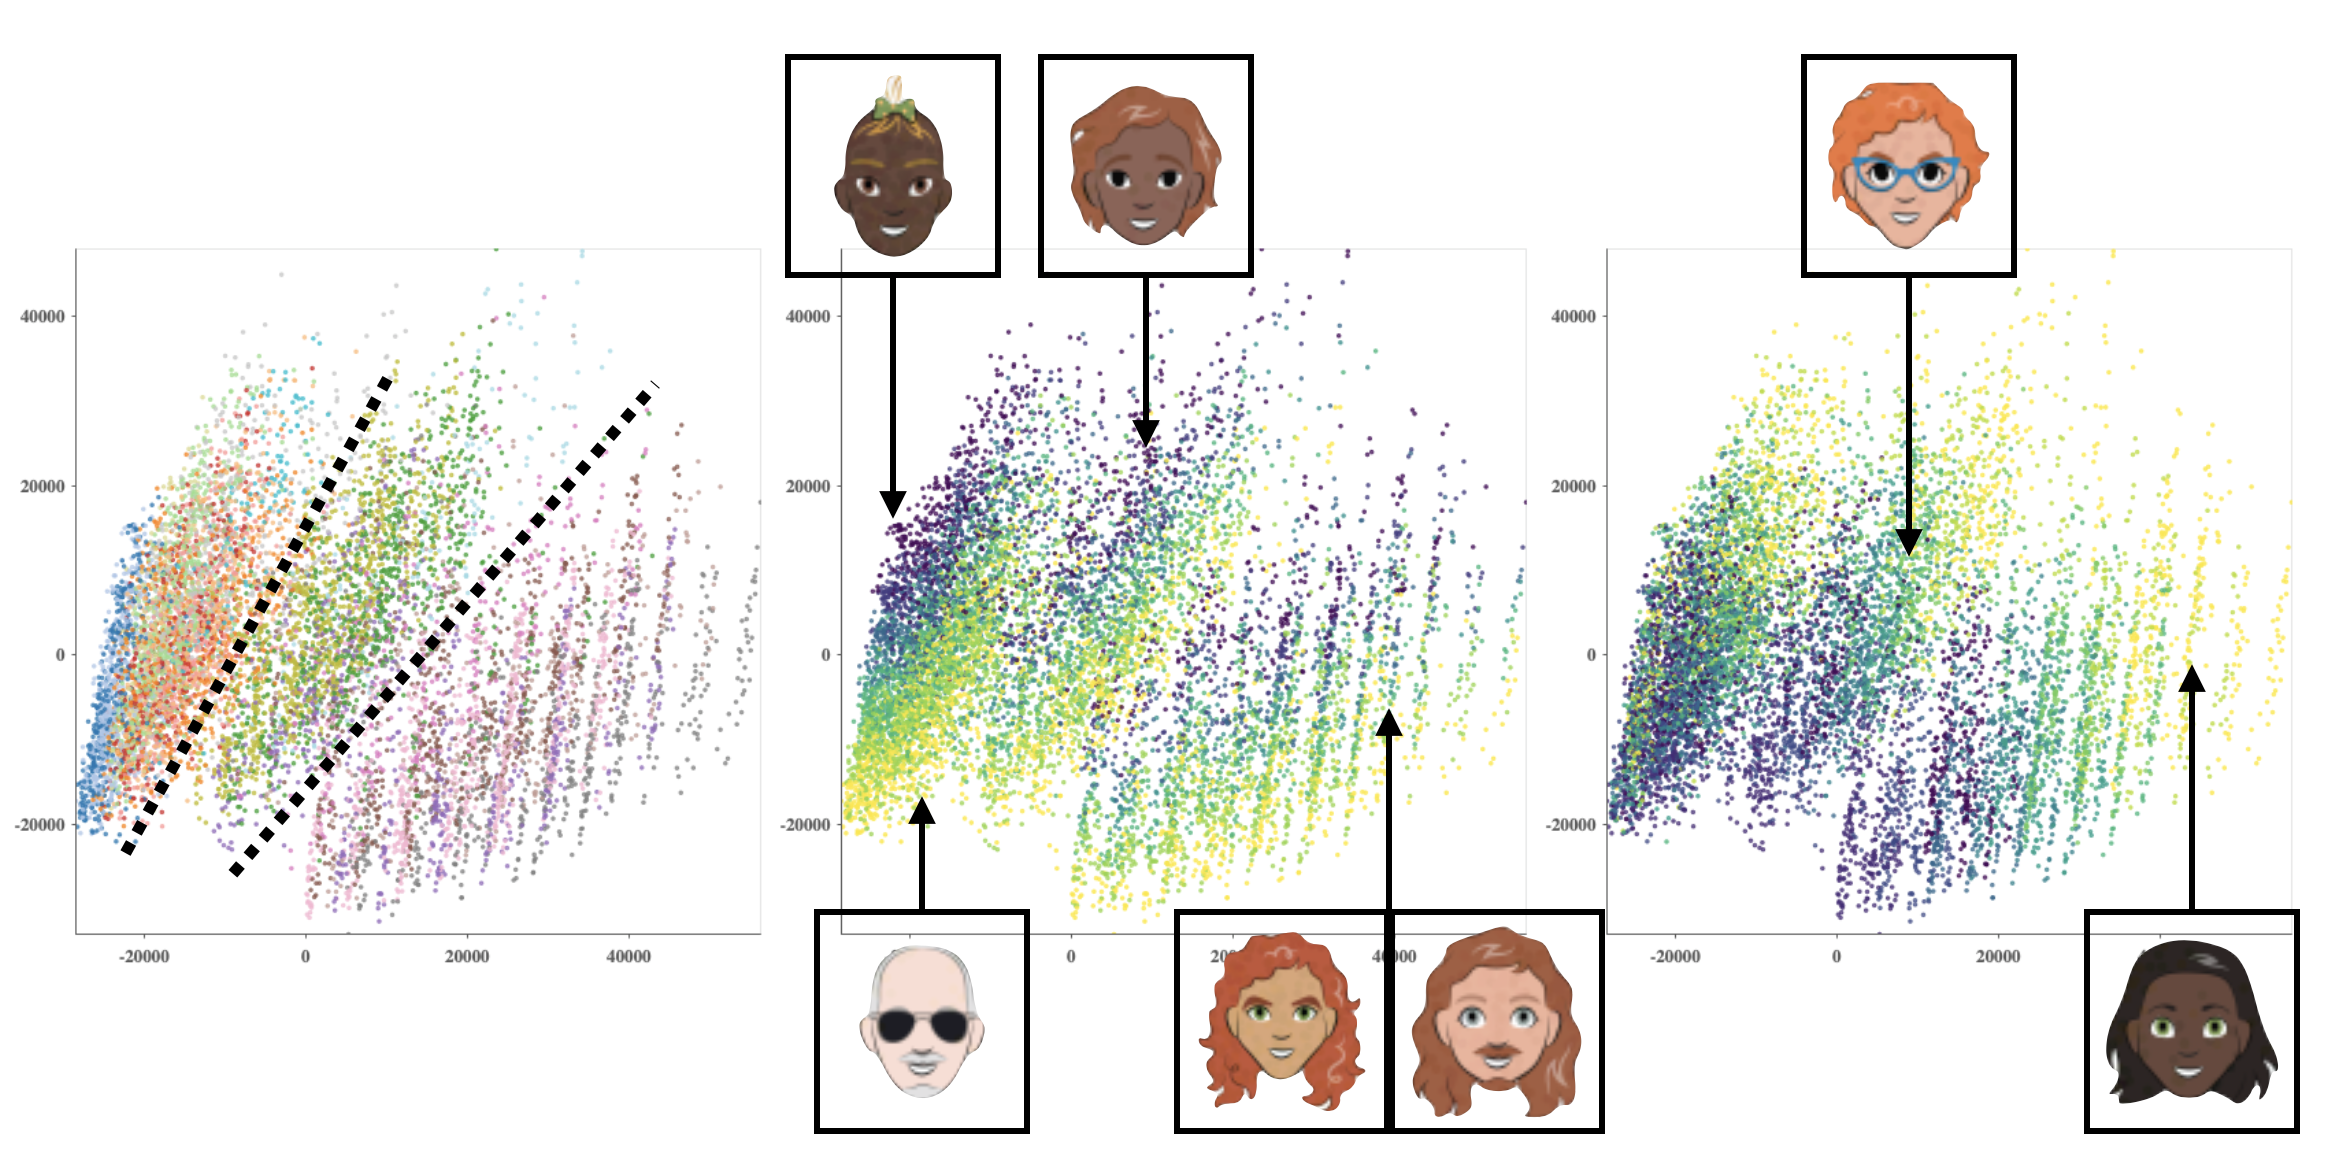
\includegraphics[width=400px, height=200px]{Figures/pca_cartoon}
		%\decoRule
		\caption[PCA auf Cartoon Set]{PCA auf dem Cartoon Set, mit $N=\num{50000}, D=\num{360000}$. 
									Dabei sind die Punkte bez�glich der folgenden Attribute gekennzeichnet (v.l.n.r): Frisurtyp, Gesichtsfarbe, Haarfarbe.}
		\label{fig:pca_cartoon}
	\end{figure}

	In Abbildung \ref{fig:cartoon_cluster} betrachten wir Einbettungen von UMAP, t-SNE und TriMap. Durch das einzeichnen der Cluster m�chten wir untersuchen, 
	wie gut die Verfahren eine \textit{globale} Struktur erhalten. Die Ergebnisse der Einbettungen unterscheiden sich stark von der PCA Einbettung. 
	Alle drei Verfahren erkennen die globale Einteilung der Daten in verschiedene Frisurtypen. Dabei unterscheiden sie zus�tzlich zu PCA innerhalb der drei Klassen, 
	kurze, mittellange und lange, in feinere Klassen. Diese entsprechen den verschiedenen Labels der Frisurtypen, wie man an den Farben der Cluster erkennen kann. 
	Dabei scheint UMAP die globale Struktur auf den ersten Blick am besten zu erkennen, da die langen und kurzen Haartypen global gro�e Abst�nde aufweisen. Allerdings 
	kann auch argumentiert werden, dass TriMap die globale Struktur am besten darstellt, da das gelbe und blaue Cluster zwar durch Haartypen mittellanger Haare getrennt 
	sind aber die Distanzen zwischen den Clustern eher flie�end sind, analog zu PCA. 
	Dies weist auf die Schwierigkeit hin, ein Ma� der globalen Qualit�t einer Einbettung zu definieren.

	\begin{figure} % Globale struktur der Punkte in den Verfahren. cmap=nhair
		%\centering
		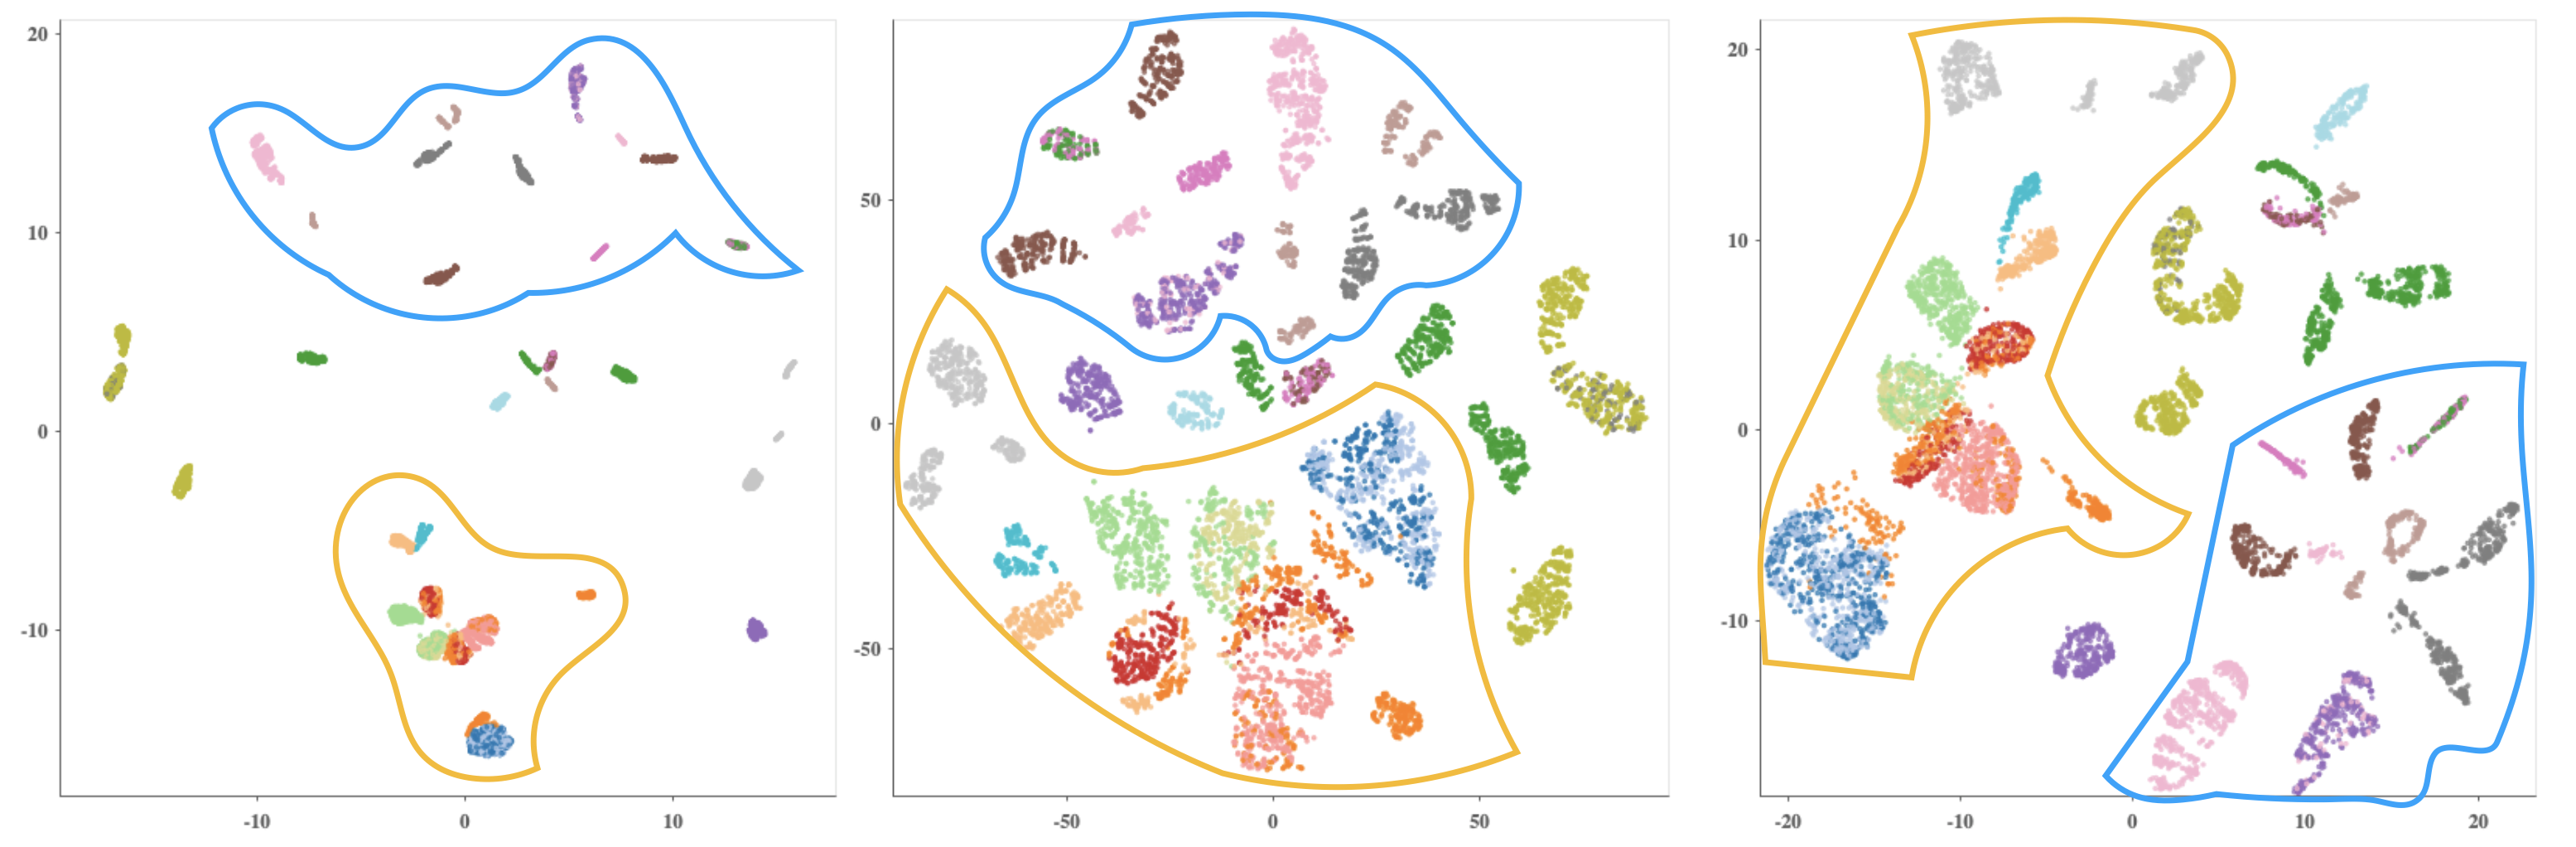
\includegraphics[width=400px, height=131px]{Figures/cartoon_cluster}
		%\decoRule
		\caption[Cluster des Cartoon Set]{(v.l.n.r) UMAP, t-SNE, TriMap auf dem Cartoon Set, mit $N=\num{50000}, D=\num{360000}$. 
										Dabei entsprechen die Punkte des gelben Gebiets dem oberen Drittel der PCA Einbettung, 
										das blaue Gebiet dem unteren Drittel der PCA Einbettung und die Punkte au�erhalb eines Gebietes dem mittleren Teil der PCA Einbettung}
		\label{fig:cartoon_cluster}
	\end{figure}

	Wir m�chten uns nun den lokalen Eigenschaften der Einbettungen zu wenden. Daf�r betrachten wir die gleiche Einbettung allerdings haben wir die Farben der Punkte diesmal 
	bez�glich der Haarfarbe, beziehungsweise der Hautfarbe gew�hlt. Den Verlauf der Farben bez�glich dieser Attribute haben wir bereits oben beschrieben. 
	Abbildung \ref{fig:cartoon_local} zeigt die von UMAP, t-SNE und TriMap erzeugte Einbettung eines Teils der Daten. 
	Wir sehen, dass alle drei Verfahren lokal die Cluster, welche die Frisurtypen 
	darstellen, als zweidimensionale Mannigfaltigkeiten auffassen. Dabei ist eine Dimension die Haarfarbe und die zweite Dimension die Hautfarbe. 
	Alle drei Plots der oberen Reihe weisen ein Cluster auf, welches anscheinend keine Struktur bez�glich der Haarfarbe aufweist. Diese Punkte beschreiben allerdings Gesichter 
	ohne Haare. 
	Die Einbettung des t-SNE Verfahrens zeigt lokal keine deutlichen Unterschiede in der Dichte. 
	Die �berg�nge zwischen den lokalen Eigenschaften in der TriMap Einbettung sind flie�ender als in der t-SNE und UMAP Einbettung. 

	\begin{figure} % Lokale struktur der Punkte in den Verfahren. cmap=nhair_color and cmap=nface_color. �berg�nge in TriMap flie�ender, tSNE weniger geh�uft/dicht als umap
		%\centering
		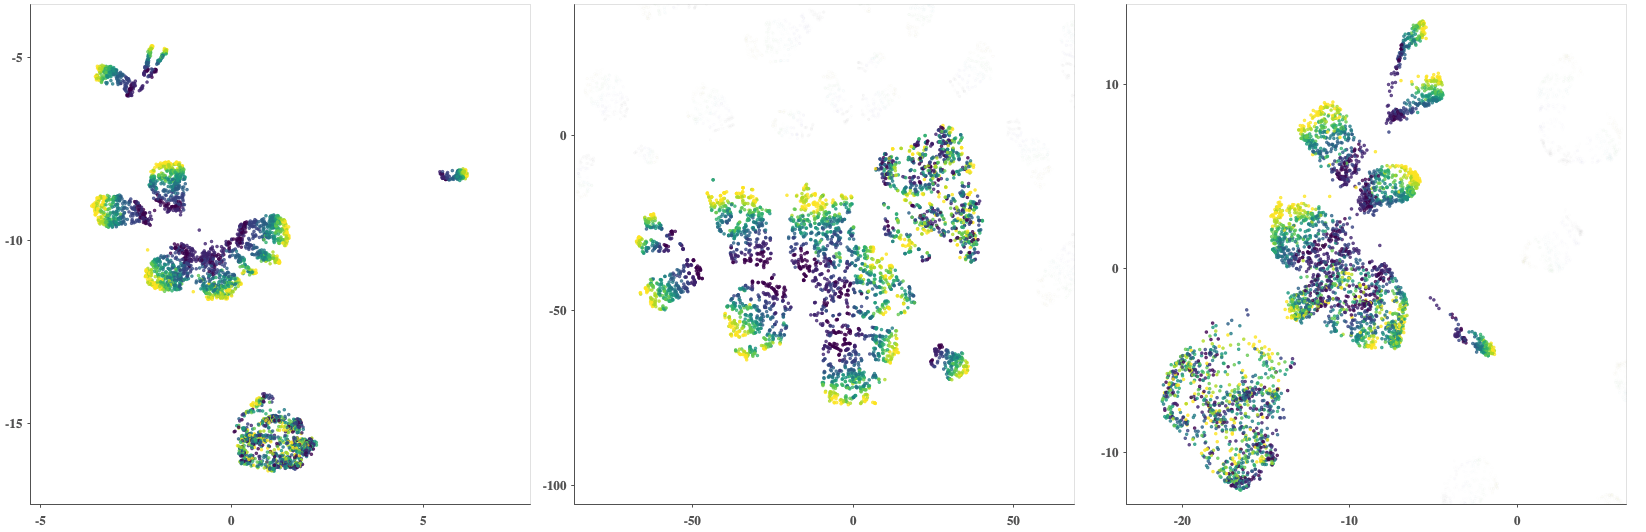
\includegraphics[width=400px, height=272px]{Figures/cartoon_local}
		%\decoRule
		\caption[Cluster des Cartoon Set]{(v.l.n.r) UMAP, t-SNE, TriMap auf dem Cartoon Set, mit $N=\num{10000}, D=\num{360000}$. 
										Die Datenpunkte der oberen Reihe sind nach der Haarfarbe und die der unteren Reihe nach der Hautfarbe gef�rbt.
										Es wurde nur ein Teil des Datensatzes betrachtet.}
		\label{fig:cartoon_local}
	\end{figure}

	Abbildung \ref{fig:cartoon_local_local} beruht auf der f�r Abbildung \ref{fig:cartoon_local} beschriebenen Einbettung. Die Farben sind bez�glich der Haarfarbe. 
	Es ist deutlich zu erkennen, dass alle drei Verfahren die Gleiche lokale Struktur f�r dieses CLuster finden. 

	\begin{figure} % Lokale struktur der Punkte in den Verfahren, cluster sehr �hnlich. cmap=nhair_color
		%\centering
		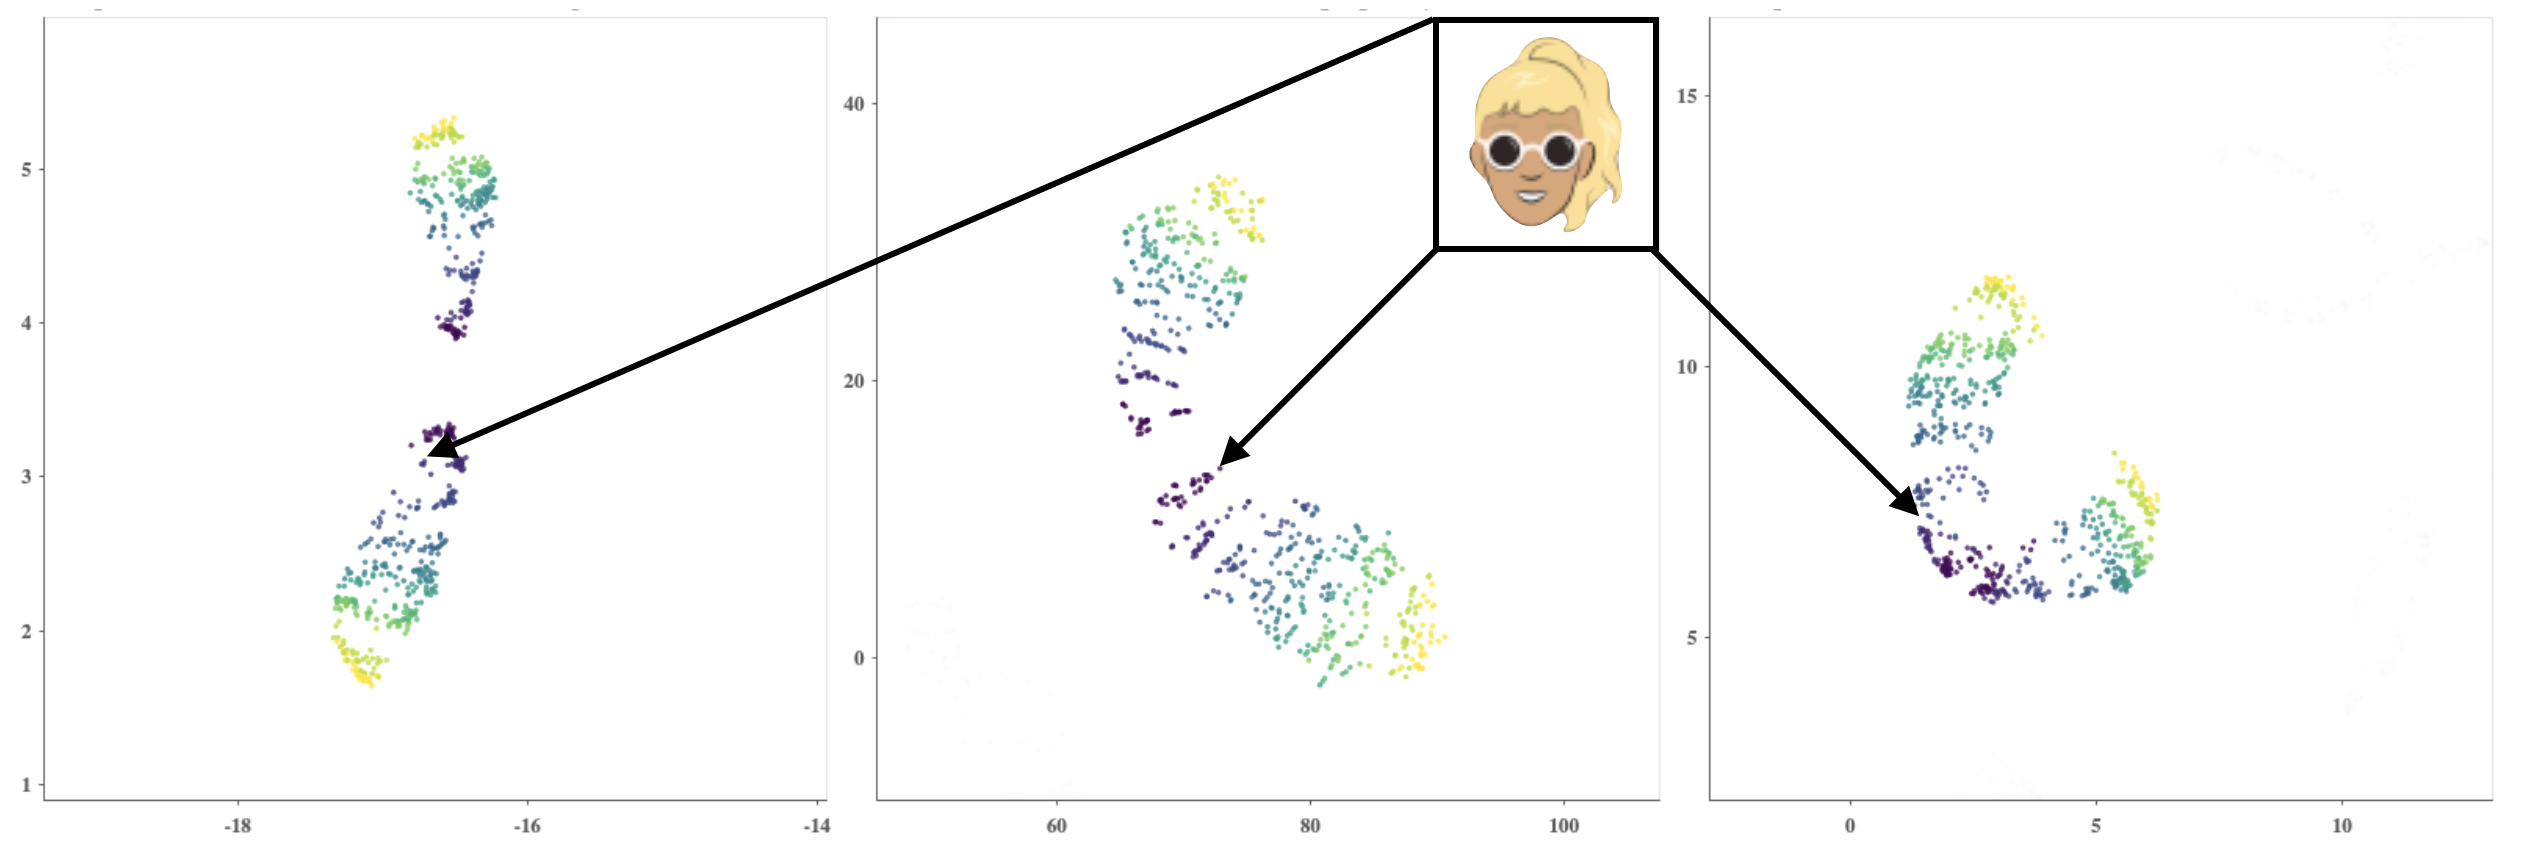
\includegraphics[width=400px, height=134px]{Figures/cartoon_local_local}
		%\decoRule
		\caption[Cluster des Cartoon Set]{(v.l.n.r) UMAP, t-SNE, TriMap auf dem Cartoon Set, mit $N=\num{50000}, D=\num{360000}$. 
										Die Position eines Datenpunktes bez�glich der verschiedenen Verfahren.}
		\label{fig:cartoon_local_local}
	\end{figure}

	Wir k�nnen festhalten, das die drei Verfahren lokal sehr �hnlich sind, die Wahl eines Verfahrens ist somit von der konkreten Anwendung abh�ngig, 
	oder im Falle der Visualisierung vom subjektiven Urteil des Betrachters. Global enth�lt die Darstellung von t-SNE sehr wenige Informationen. 
	Das UMAP und TriMap Verfahren erhalten globale Eigenschaften, dabei ist der Begriff \textit{global} allerdings nicht formal gegeben und sollte 
	genauer untersucht werden. 

%----------------------------------------------------------------------------------------

\section{MNIST} \label{sec:FMNIST}
	Wir m�chten kurz die Einbettungen der Verfahren auf dem MNIST Datensatz zeigen. Dieser besteht aus Bildern der Gr��e $28 \times 28$, welche 
	die Ziffern von $0$ bis $9$ darstellen. Dabei ist zu erkennen, dass alle nicht linearen Verfahren $10$ Cluster erkennen. 
	Das UMAP Verfahren spiegelt die mittels PCA gefundene globale Struktur am besten wieder. Dabei ist auch zu erw�hnen, dass TriMap eine gewisse 
	globale Struktur darstellt, da es das blaue Cluster (Ziffer 1), das pinke, t�rkise und orange Cluster (Ziffern 7, 4, 9) und die restlichen 
	Cluster von einander separiert. 
	Zus�tzlich ist zu erkennen, das die Cluster von openTSNE separierter von einander sind, als die vom tSNE Verfahren, dies ist auf die Implementierung 
	des \code{late-exaggeration} Parameters im openTSNE Code zur�ckzuf�hren.
	% Lokal gut Einbettung vergleichbar mit anderen Verfahren
	% variiere set_opt_mix
	% Beispielsweise sollten die Cluster welche die Ziffern 1 und 7 darstellen n�her zueinander liegen als die Cluster der Ziffern 1 und 6. 

	\begin{figure} % Lokale struktur der Punkte in den Verfahren. cmap=nhair_color and cmap=nface_color. �berg�nge in TriMap flie�ender, tSNE weniger geh�uft/dicht als umap
		%\centering
		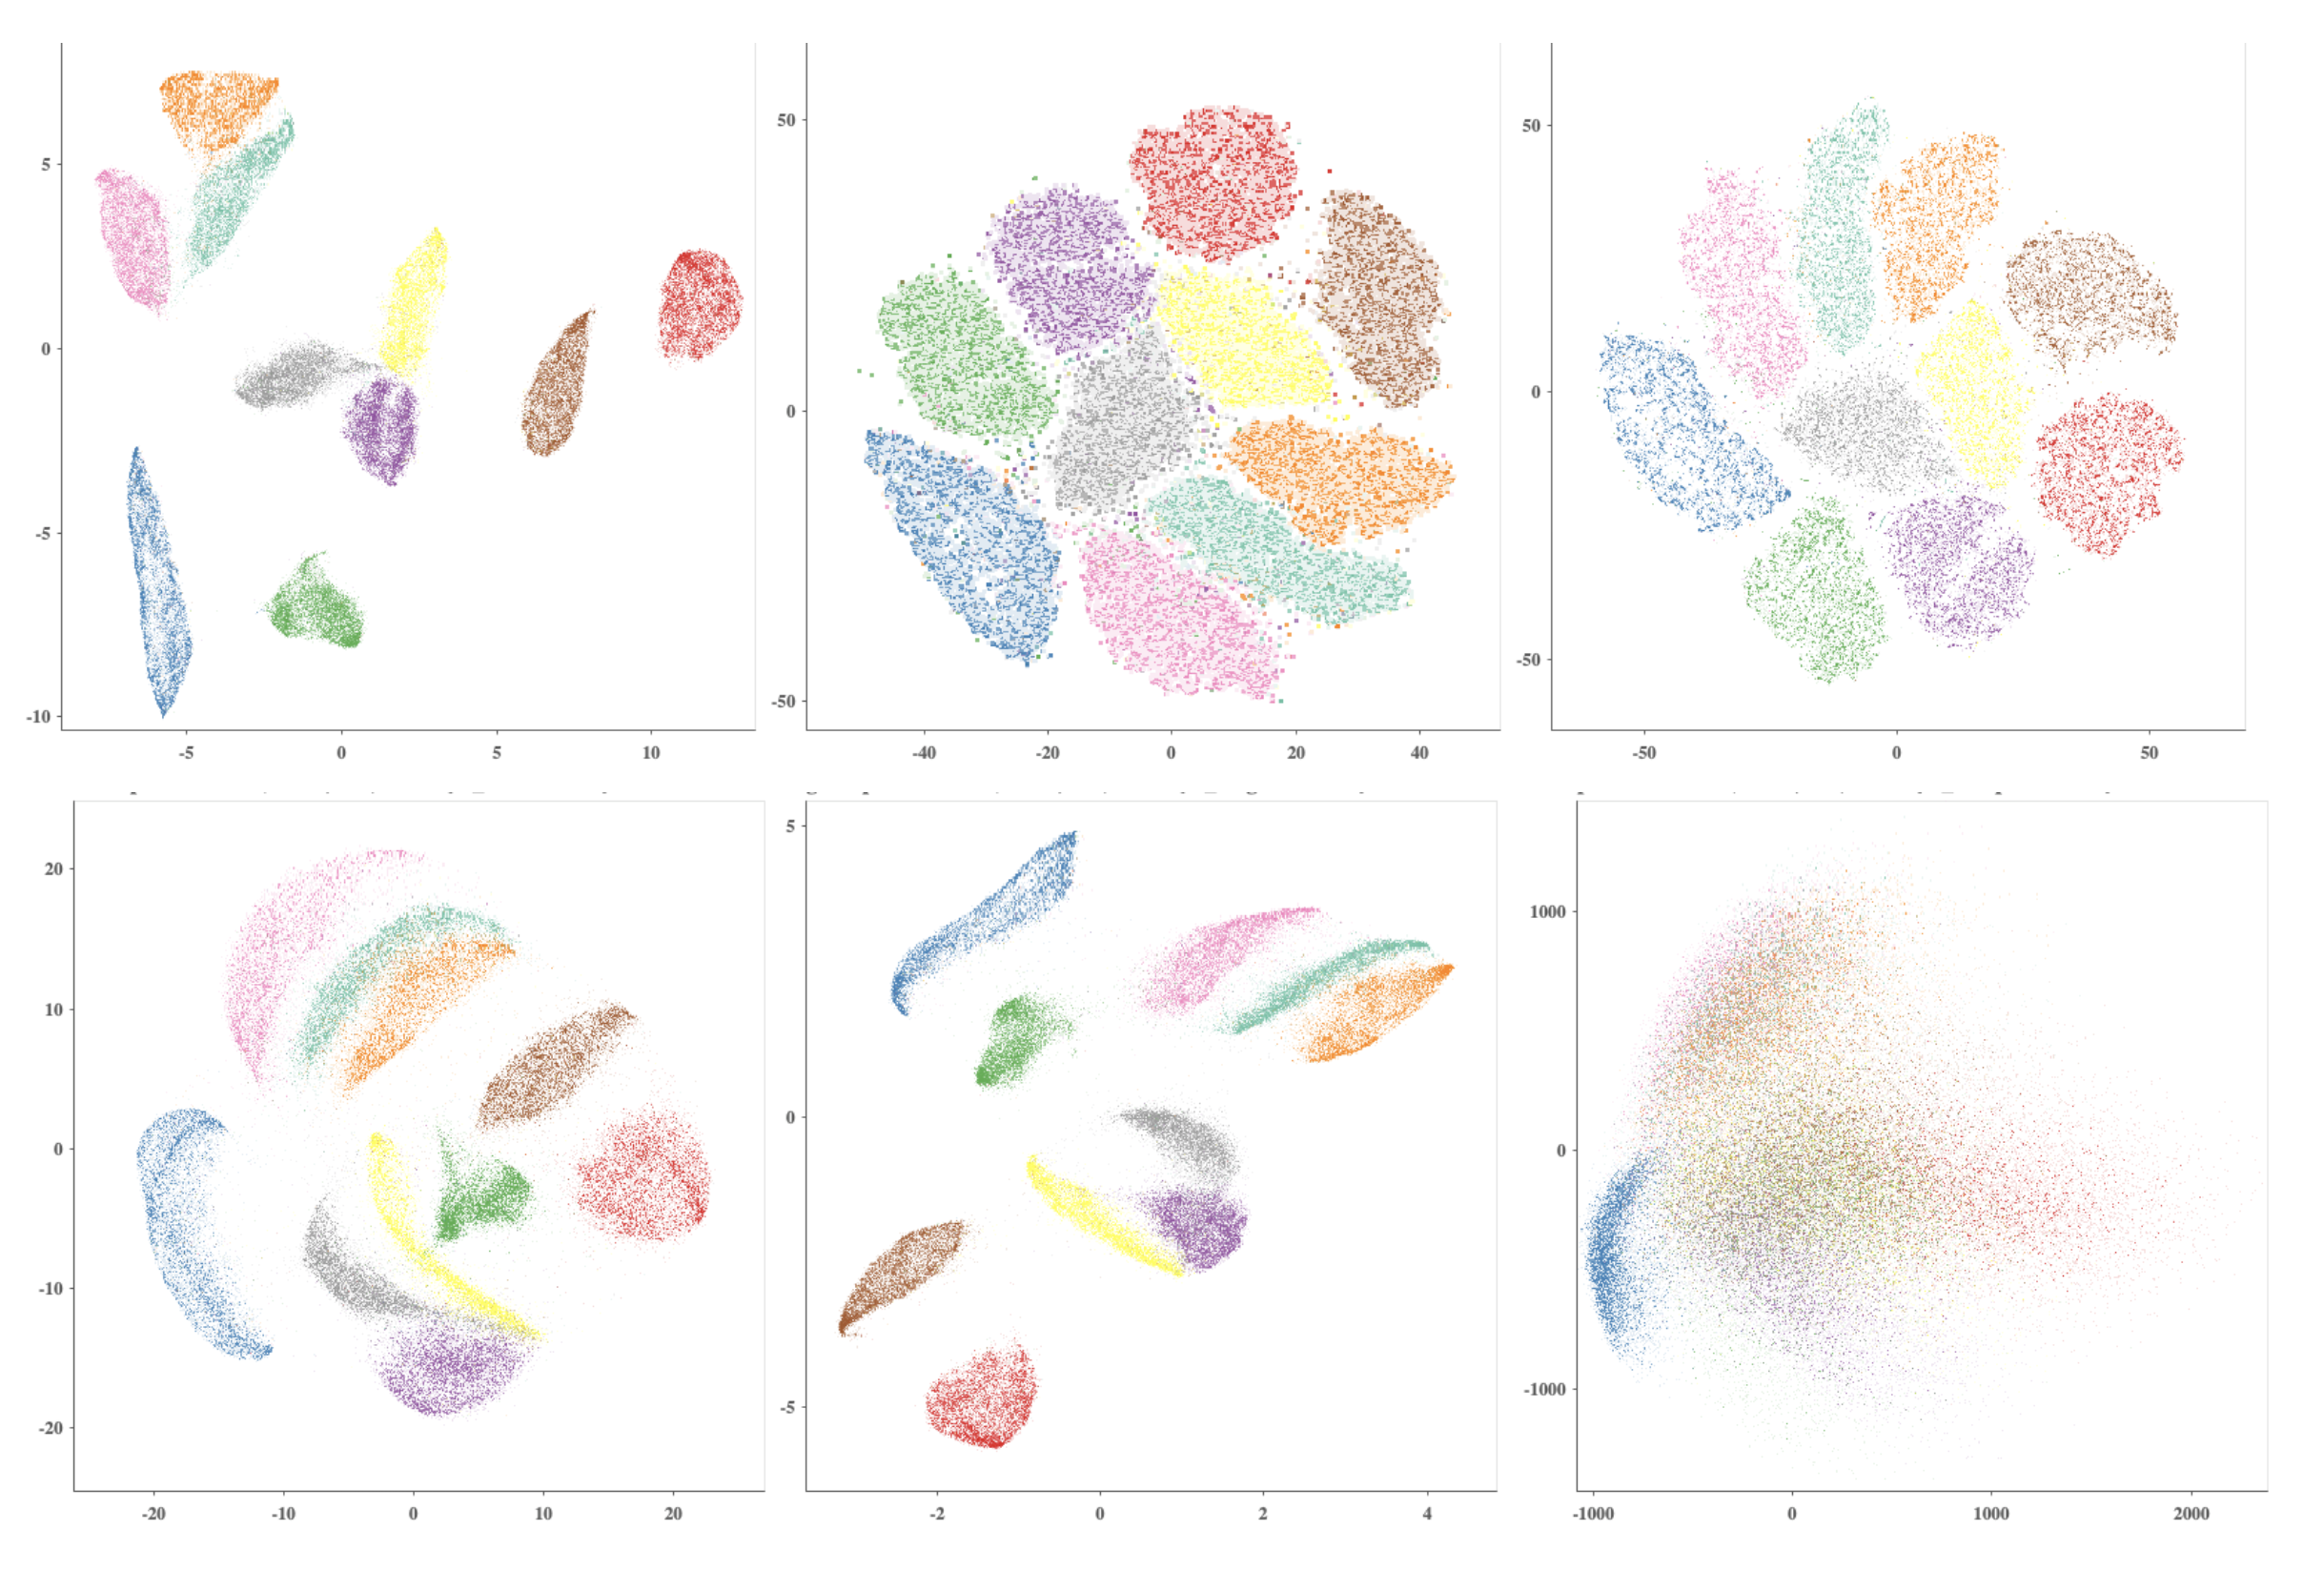
\includegraphics[width=400px, height=300px]{Figures/FMNIST}
		%\decoRule
		\caption[Cluster FMNIST]{(oben v.l.n.r) UMAP, t-SNE, OpenTSNE auf FMNIST, mit $N=\num{70000}, D=\num{784}$. 
									(unten v.l.n.r) TriMap, GPU UMAP, PCA}
		\label{fig:FMNIST}
	\end{figure}
	
%----------------------------------------------------------------------------------------

\section{Laufzeitanalyse} \label{sec:runtime}
	Die praktischen Tests der Verfahren wurden auf Rechnern mit einer Linux-Architektur ausgef�hrt. 
	Die CPU Tests haben wir auf Intel Xeon 6136 CPUs mit 48 Kernen und 384 GB RAM ausgef�hrt. 
	F�r die Verfahren welche mittels Berechnungen auf einer Graphikkarte verbessert wurden, haben 
	wir Intel Xeon Gold 6136 CPUs mit 188 GB RAM und Nvidia V100 GPUs genutzt. 
	In Tabelle \ref{tab:umap} stellen wir die Laufzeit von UMAP abh�ngig vom \code{n\_neighbors} 
	Parameter da. Die Laufzeit des Verfahrens erh�ht sich um den Faktor $8x$, wenn der Parameter 
	von 5 auf 100 erh�ht wird. Dies spiegelt die in Abschnitt \ref{sec:profile} gemachte Aussage 
	wieder, dass das NN-Descent Verfahren zur Nachbarschaftssuche eine Schwachstelle im UMAP Verfahren ist. 
	Betrachtet man die Laufzeit der GPU Implementierung \cite{GPUUMAP} auf dem FMNIST Datensatz, 
	so erh�ht sich die Laufzeit von 2,63 Sekunden auf 3 Sekunden. 
	Leider konnten wir die GPU Implementierung nicht auf dem vollen Cartoon Set testen, da die 
	aktuelle Version den Datensatz in den GPU Arbeitsspeicher l�dt. Wir hatten nur $16$ GB GPU RAM 
	zur Verf�gung, dies hat f�r die hohe Dimension des Cartoon Set nicht ausgereicht hat. 
	Um dennoch das GPU Verfahren mit h�her dimensionalen Daten zu testen, haben wir das Cartoon Set 
	zu erst mit PCA auf 784 Dimensionen vorverarbeitet, die Laufzeit auf dem vorverarbeiteten Datensatz 
	variierte zwischen 4 Sekunden und 7,4 Sekunden. 

	\begin{table}
	\centering
	\begin{tabular}{l|llll}
	\code{n\_neighbors} & MNIST    & FMNIST & Cartoon 10k & Cartoon 50k \\ \hline
	5    				& 3,7 min  & 4 min  & 7,4 min     & 62 min      \\
	10   				& 5,3 min  & 6 min  & 11,4 min    & -           \\
	20   				& 10,6 min & 12 min & 23 min      & -           \\
	40   				& 25 min   & 24 min & 77 min      & 7 h         \\
	100  				& 34 min   & 32 min & 86 min      & 8 h        
	\end{tabular}
	\caption{Laufzeit des UMAP Verfahren mit unterschiedlichen Werten des \code{n\_neighbors} Parameters.}
	\label{tab:umap}
	\end{table}

	Nat�rlich m�chten wir die Laufzeit des UMAP Verfahrens auch mit der von anderen Verfahren vergleichen, 
	dazu haben wir drei Implementierungen des t-SNE Verfahrens betrachtet, das oben beschriebene TriMap 
	Verfahren und PCA. 

	\begin{table}
	\centering
	\begin{tabular}{l|lll}
	           & MNIST    & FMNIST   & Cartoon 10k \\ \hline
	UMAP       & 25 min   & 23,8 min & 77 min      \\
	t-SNE      & 2 h      & 130 min  & 17 h        \\
	openTSNE   & 11,6 min & 12 min   & -           \\
	TriMap     & 4 min    & 4 min    & 5,4 min     \\
	Cuda UMAP  & 8 sec    & 7,7 sec  & -           \\
	Cuda t-SNE & 5 sec    & 5,4 sec  & -           \\
	PCA        & 1,3 sec  & 1,2 sec  & 9,2 min    
	\end{tabular}
	\caption{Laufzeit verschiedener Verfahren der Dimensionsreduktion}
	\label{tab:several}
	\end{table}

	Wir k�nnen somit festhalten, dass die GPU Implementierungen aufgrund ihrer 
	Laufzeit f�r Zwecke genutzt werden k�nnen, wo bisher nur einfache lineare DR Verfahren 
	wie PCA genutzt werden konnten. 
	Die TriMap Implementierung ist das schnellste nicht-lineare CPU DR Verfahren, welches 
	wir betrachtet haben. Insbesondere skaliert es sehr gut in der Umgebungsdimension, 
	wobei wir hervor heben m�chten, dass es auf dem Cartoon Set mit $N = \num{10000}, D = \num{360000}$ 
	schneller als PCA war. Somit scheint eine ausf�hrlichere Betrachtung des TriMap Verfahrens 
	aufgrund seiner Laufzeit und Qualit�t der Ergebnisse sinnvoll zu sein. 

%----------------------------------------------------------------------------------------
%!TEX root = ../main.tex

\chapter{Zusammenfassung und Ausblick} 

\label{Zusammenfassung}

%----------------------------------------------------------------------------------------

% Problem mit rauschenden Daten: nutze random projections (~siehe Tang)

% Anwendung wo Mannigfaltigkeitshypothese nicht wahr ist siehe Oudot s.68
% Bildausschnitte, Sensordaten,...

% Keine genaue Interpretation über Dimensionen

% Lokale Eigenschaften sind wichtiger als globale

% Metric Learning 54, 7

% Durch lokale Eigenschaft sind die resultierenden Cluster ähnlich groß, 
% unabhängig von der Ausgangsgröße

% Was sind die stärken was sind die schwächen?

% Aufgrund der schnellen Implementierung auf dem GPU ist eine Interaction mit dem Nutzer 
% möglich \cite{Verleysen} sieht dies als wichtigen Punkt für DR Algorithmen
% (siehe https://perso.uclouvain.be/michel.verleysen/papers/iconip13mv.pdf)
% gemeinsam mit online kNN
% (siehe: https://arxiv.org/pdf/1804.03032.pdf)

%----------------------------------------------------------------------------------------

% Anwendung auf andere Datensätze Beispielsweise Kundendatenbank, als Vorverarbeitung, 
% Zeitreihenanalyse

% Höhere Simplizes betrachten (siehe Methoden von TriMap)

% Verfahren zum finden der zugrundeliegenden Dimension, kann variieren (=> variierender 
% near_neighbor Parameter?)

% UMAP zur Gesichtserkennung (siehe Eigenfaces)

% “Product quantization for nearest neighbor search”, Jegou & al., PAMI 2011.
% Zur Darstellung hochdimensionaler Vektoren
% This can be seen as a lossy compression technique for high-dimensional vectors, 
% that allows relatively accurate reconstructions and distance computations in the compressed domain.

% Betrachten einer Umkehrabbildung

% Erwähne smallvis (und 'schnellere' uwot version) für SGD ohne sub sampleing
% Da wir uns in den Experiementen auf die DR mittels schneller Implementierungen für 
% große Datensätze fokussiert haben, sind diese beiden Implementierungen nicht erwähnt..

% TODO: Beschreibung der Lücke in diesem Kapitel oder in UMAP

% Wie kann man Daten besser vorverarbeiten um die Ergebnisse noch zu verbessern?

%----------------------------------------------------------------------------------------
%---------------------------------------------------------------------------------------- 

%----------------------------------------------------------------------------------------
%	THESIS CONTENT - APPENDICES
%----------------------------------------------------------------------------------------

\appendix % Cue to tell LaTeX that the following "chapters" are Appendices

% Include the appendices of the thesis as separate files from the Appendices folder
% Uncomment the lines as you write the Appendices

%%!TEX root = ../main.tex

\chapter{Appendix A}

\label{AppendixA}

% Bisher: Daten -> metr. R�ume -> fuzzy simplicial sets
% Ziel:   Daten -> metr. R�ume -> VR complex

% Wenn VR Komplex ausreichend, betrachte nur 1-Skelet und berechne Homologie darauf.
% Siehe Oudot s.48, funktioniert noch nicht f�r Filtrationen. 

%----------------------------------------------------------------------------------------

% TODO: evtl Cech und VR in Grundlagen
\section{Homologie}
	% Hom�omorphismus, Homologie (Gruppen), homologie Equivalenz,
	Eine bekannte Aussage, welche der Topologie entstammt, ist, dass eine Kaffeetasse das Gleiche \textit{topologische Objekt} 
	wie ein Donut ist. Dies ist dadurch begr�ndet, dass man eine Kaffeetasse durch strecken und stauchen 
	(ohne rei�en) in einen Donut transformieren kann. Diese \textit{Gleichheit} l�sst sich wie folgt mathematisch darstellen:

	\begin{defn}[Stetige Abbildung]
		Sei ...
	\end{defn}

	\begin{defn}[Hom�omorphismus]
		Sei ...
	\end{defn}

	Nun werden wir den Begriff der Homologie einf�hren. Daf�r werden wir den Begriff der simplizialen Komplexe 
	ben�tigen um zuerst die simpliziale Homologie einzuf�hren.

	\begin{defn}[Simplizialer Komplex]
		Sei ...
	\end{defn}

	\begin{defn}[Abstrakter simplizialer Komplex]
		Sei ...
	\end{defn}

	\begin{ex}
		\cech-Komplex
	\end{ex}

	\begin{ex}
		VR-Komplex
	\end{ex}

	\begin{defn}[Homologie]
		Sei ...
	\end{defn}

	\begin{defn}[Homologiegruppe]
		Sei ...
	\end{defn}

	\begin{ex}
		Die Homologiegruppen eines Balls, Donuts, Graphen, ...
	\end{ex}

	\begin{defn}[Filtration]
		Sei $T \subseteq \R$, eine \textit{Filtration} $\mathcal{X}$ �ber $T$ ist eine Familie von 
		topologischen R�umen $\{X_i\}_{i \in T}$, so dass $X_i \subseteq X_j$ 
		f�r $i \leq j \in T$.  % (Oudot s.29)
	\end{defn}

	\begin{rem}
		Eine Filtration $\mathcal{X}$ wird meist nicht als Familie verschiedener topologischer 
		R�ume $X_i$ angesehen, sondern als ein einziger Raum, welcher sich im Laufe der Zeit 
		\enquote{transformiert}. Siehe dazu \cite{Oudot}.  % (Oudot s.30)
		Dies stimmt mit unserem Bild �berein, den $\epsilon$-Parameter eines \cech-Komplexes %TODO: Satz l�schen und motivation cech komplex nennen
		immer gr��er werden zu lassen. Wir werden \textit{persistente Homologie} nutzen um 
		die homologischen Eigenschaften zu beschreiben, welche f�r alle $i \in T$ erhalten 
		(bzw. persistent) bleiben.
	\end{rem}

	% TODO: Oudot Kap. 4,5 f�r Anwendungen von persistenter Homologie

	% TODO: Bemerkung, dass \mathcal{X} eine Repr�sentation eines Poset ist (siehe Oudot s.29)

	\begin{ex}
		% TODO: warum?
		Insbesondere ist somit der \cech-Komplex eine Filtration, da ...
	\end{ex}

	\begin{ex}
		% TODO: warum?
		Eine weitere Filtration ist der Vietoris-Rips-Komplex
	\end{ex}

	\begin{rem} % TODO: Bem in Def umwandeln
		Der VR-Komplex ist ein Beispiel eines Clique-Komplexes und wird als solcher 
		eindeutig durch sein 1-Skelet identifiziert. Sei $V$ ein VR-Komplex und $V^1$ das 
		zugeh�rige 1-Skelet. Dann erh�lt man $V$ aus $V^1$, indem man alle Cliquen im 
		$V^1$ zugrundeliegenden Graphen bestimmt. Eine k-Clique ist ein vollst�ndiger Subgraph 
		mit k Knoten. 
	\end{rem}

	Es gibt weitere Formen von Komplexen, die bekanntesten sind die CW-Komplexe und Zellkomplexe. 
	Ziel ist es stets mit Hilfe einfacher Konstrukte die Topologie eines Raums zu beschreiben.

	Die vom \cech-Komplex und vom Vietoris-Rips-Komplex beschriebene Homologie kann sich unterscheiden (siehe Abbildung \ref{fig:Cech_VR}).

	\begin{figure}
		%\centering
		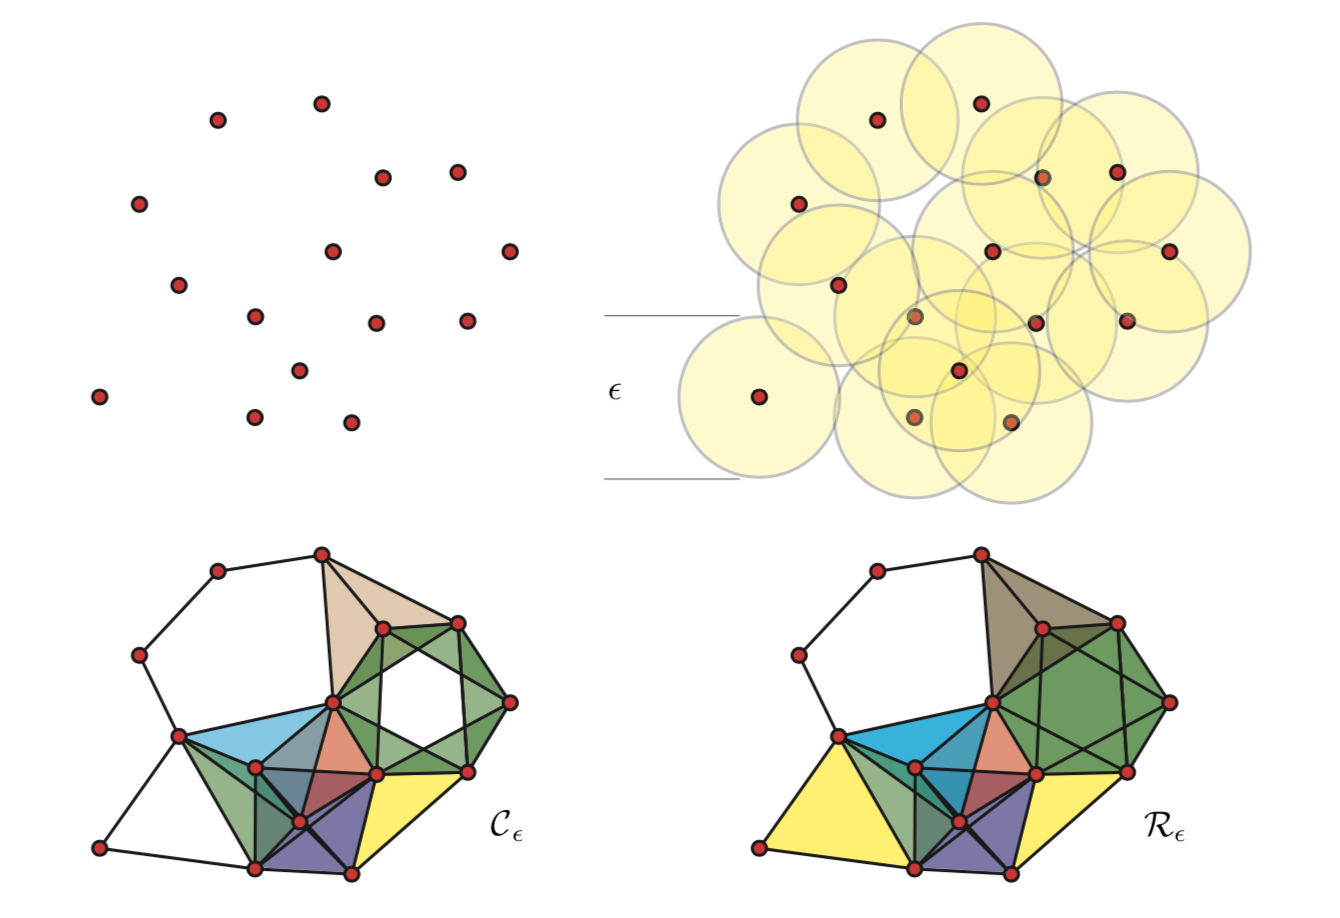
\includegraphics[width=400px, height=274px]{Figures/Cech_VR_complex}  % width=1\textwidth
		%\decoRule
		\captionsetup{justification=RaggedRight}  % centerfirst
		\caption[Versch. Komplexe]{Eine Punktwolke [oben links] kann zu einem \cech-Komplex [unten links] 
								   oder einem VR-Komplex [unten rechts] basierend auf dem Parameter $\epsilon$ 
								   konstruiert werden. Die Homotopietypen der $\epsilon/2$ �berdeckung vom 
								   \cech-Komplex ($S^1 \vee S^1 \vee S^1$), w�hrend das VR-Komplex die Homotopietypen 
								   ($S^1 \vee S^2$) besitzt. (\textit{Quelle:} \cite{Barcodes})}

		\label{fig:Cech_VR}
	\end{figure}

	Wir ben�tigen nun noch den Begriff einer \textit{guten �berdeckung} um dann eine geeignete Aussage �ber einen \cech-Komplex einer Menge zu machen. 

	\begin{defn}[�berdeckung]
		Eine �berdeckung eines topologischen Raumes ist \dots
		Eine gute �berdeckung ist \dots
	\end{defn}

	\begin{NT}  % Nerv Theorem
		% Ein top. Raum ist homotopie equivalent zu einer endlichen guten �berdeckung. 
		Sei ...
		\label{thm:NT}
	\end{NT}
	
	Das Nerv Theorem \ref{thm:NT} liefert uns eine Aussage dar�ber, dass ein topologischer Raum $X$ zu einer endlichen guten 
	�berdeckung von $X$ homotopie�quivalent ist.
	Wie wir sehen ist die Konstruktion stark abh�ngig vom $\epsilon$-Parameter. Um dem 
	entgegenzuwirken nutzt man die Idee der \textit{persistenten Homologie}. Dabei 
	wird betrachtet wie sich die Homologie eines Raumes f�r eine monoton wachsende Folge 
	$(\epsilon_i)_{i \in \N}$ verh�lt.

	F�r den von uns betrachteten Fall, die Struktur einer Riemannschen Mannigfaltigkeit $(\M, g)$ zu beschreiben, werden wir 
	Annehmen, dass die Daten $\mathbf{x}_i \in X$ gleichverteilt bez�glich der Riemannmetrik $g$ sind, bzw. $g$ so w�hlen, das 
	die Annahme erf�llt ist. Somit erhalten wir eine gute �berdeckung ohne eine Abh�ngigkeit von $\epsilon$ zu haben. 

%%!TEX root = ../main.tex

\chapter{Appendix B} \label{AppendixB}


%----------------------------------------------------------------------------------------


   % Um eine Unterscheidung zwischen der theoretischen Sichtweise auf das UMAP Verfahren, welche alle $k$-Simplizes 
   % $(1 \leq k \leq N)$ ber�cksichtigt, und der praktischen Implementierung zu verdeutlichen, werden wir die 
   % verwendete Notation anpassen. 

   % Die unsicheren Mengen $(A, \mu), (A, \nu)$ aus Gleichung (\ref{eq:crossentropy}) lassen sich als gewichtete Graphen, 
   % in Form einer Adjazenzmatrix darstellen. % TODO: F�r den Fall, dass nur 1-Simplizes betrachtet werden
   % Das 1-Skelett der hochdimensionalen Repr�sentation notieren wir als Adjazenzmatrix $V$ mit $\vij = \mu(a)$, f�r 
   % ein 1-Simplex $a$, mit Facetten $i$ und $j$. 
   % % TODO: Wahl von \vij

   % Die Wahl des Zugeh�rigkeitsgrades f�r 1-Simplizes der niedrigdimensionalen Repr�sentation der Daten ist wie folgt gegeben:

   % \begin{equation}
   %    \wij = (1+a(\norm{\mathbf{y}_i - \mathbf{y}_j}^2_2)^b)^{-1}, \label{eq:wij} % TODO: wie sind a, b gew�hlt?
   % \end{equation}

   % % TODO: f�r a=b=1 tSNE, b=1 LargeVis

   % wobei $\mathbf{y}_i, 1 \leq i \leq N$ die Vektoren der Einbettung sind. Die Wahl der Werte $a,b$ werden wir in 
   % Abschnitt \ref{seq:hyper} beschreiben.


   % Somit erhalten wir folgende Kreuzentropie zwischen den Graphen der hoch- und niedrigdimensionalen 
   % Darstellung der Daten:

   % \begin{alignat}{2}
   %    C(V, W) &= \sumtup{i}{j} \vij \log\left(\frac{\vij}{\wij}\right) + (1-\vij) \log\left(\frac{1-\vij}{1-\wij}\right) \\
   %            &= \begin{aligned}[t]
   %                   &  \sumtup{i}{j} (\vij \log(\vij) + (1-\vij) \log(1-\vij)) \\
   %                   &- \sumtup{i}{j} (\vij \log(\wij)) - \sumtup{i}{j} ((1-\vij) \log(1-\wij))
   %                \end{aligned} \\
   %            &=  C_v - \sumtup{i}{j} (\vij \log(\wij) + (1-\vij) \log(1-\wij)) \label{eq:loss}
   % \end{alignat}

   % Der Term $C_v$ bleibt w�hrend der Minimierung der Funktion bez�glich der $\mathbf{y}_i$ konstant.
   
   % Aufgrund der Wahl einer differenzierbaren Funktion f�r den Zugeh�rigkeitsgrad der 1-Simplizes, 
   % bzw. der Gewichte des niedrigdimensionalen Graphen, l�sst sich nun der Gradient der Zielfunktion (\ref{eq:loss}) herleiten.

   % Mittels der Kettenregel ergibt sich mit $d_{ij} \coloneqq \norm{\mathbf{y}_i - \mathbf{y}_j}_2$:

   % \begin{align}
   % \quad
   %    \deriv{C}{\mathbf{y}_i} &= \sumtup{k}{l} \deriv{C}{w_{kl}} \sumtup{m}{n} \deriv{w_{kl}}{d^2_{mn}} \sumtup{p}{q} \deriv{d^2_{mn}}{d_{pq}} \deriv{d_{pq}}{\mathbf{y}_i} \\
   %                   &= \sumtup{k}{l} \deriv{C}{w_{kl}} \sumtup{m}{n} \deriv{w_{kl}}{d^2_{mn}} \deriv{d^2_{mn}}{d_{mn}} \deriv{d_{mn}}{\mathbf{y}_i} \\
   %                   &= 2 \sumtup{k}{l} \deriv{C}{w_{kl}} \sumtups{m} \deriv{w_{kl}}{d^2_{mi}} \deriv{d^2_{mi}}{d_{mi}} \deriv{d_{mi}}{\mathbf{y}_i} \\
   %                   &= 2 \sumtups{m} \left( \sumtup{k}{l} \deriv{C}{w_{kl}} \deriv{w_{kl}}{d^2_{mi}} \right) \deriv{d^2_{mi}}{d_{mi}} \deriv{d_{mi}}{\mathbf{y}_i}  \label{eq:deriv-2}\\
   %                   &= 4 \sumtups{m} \left( \sumtup{k}{l} \deriv{C}{w_{kl}} \deriv{w_{kl}}{d^2_{mi}} \right) (\mathbf{y}_i - \mathbf{y}_m) \label{eq:deriv-1}
   % \end{align}

   % Bei der Umformung von (\ref{eq:deriv-2}) nach (\ref{eq:deriv-1}) haben wir verwendet, dass $d_{mi}$ die euklidische Norm ist. 
   % F�r Einbettungen in andere metrische R�ume m�sste der Gradient an dieser Stelle entsprechend angepasst werden. Da wir 
   % das UMAP Verfahren im wesentlichen zur Visualisierung im $\R^2$ benutzen ist die Wahl der euklidischen Norm gerechtfertigt.
   % Die �brigen Umformungen ergeben sich aus umordnen und wegfallen der Terme. 

   % (\ref{eq:deriv-1}) l�sst sich weiter umformen, dazu nutzen wir:

   % \begin{align}
   %    \deriv{C}{\wij} &= - \frac{\vij}{\wij} + \frac{1-\vij}{1-\wij} = \frac{\wij - \vij}{\wij (1 - \wij)} \\
   %    \deriv{\wij}{d^2_{ij}} &= -bad_{ij}^{2(b-1)} \wij^2 = - \frac{b}{d_{ij}^2} \wij (1 - \wij)
   % \end{align}

   % Der UMAP Gradient ist also gegeben durch:
   % % TODO: Daniel: Fehlt da nicht noch eine innere Summe aus 4.9?
   % \begin{equation}
   %    \deriv{C}{\mathbf{y}_i} = 4 \sumtups{j} (\wij - \vij) \frac{b}{d_{ij}^2} (\mathbf{y}_i - \mathbf{y}_j)
   %    \label{eq:umapgrad}
   % \end{equation}
%\include{Appendices/AppendixC}

%----------------------------------------------------------------------------------------
%	BIBLIOGRAPHY
%----------------------------------------------------------------------------------------

\printbibliography[heading=bibintoc]

%----------------------------------------------------------------------------------------

%----------------------------------------------------------------------------------------
%	HELP
%----------------------------------------------------------------------------------------
%
% Bibliography not showing? Run pdflatexmk
%


\end{document}  
